\documentclass{officialexam} 

  \begin{document}
 {\maketitle}
  \borderline{វិញ្ញាសាទី១ ({\kn បាក់ឌុបឆ្នាំ ២០១៧ ថ្នាក់សង្គម})}
  
  \begin{enumerate}[I]
  \item គណនាលីមីត៖
\begin{enumerate}[k,3]
\item $\lim_{x\to +\infty}\frac{x^2+x+1}{x^2+1}$
\item $\lim_{x\to 3}\frac{x^3-27}{\sqrt{x+6}-3}$
\item $\lim_{x\to 0}\frac{e^x+e^{-x}}{2}$
\end{enumerate}
\item ក្នុងថង់មួយមានប៊ូលពណ៌សចំនួន៣ និងប៊ូលពណ៌ក្រហមចំនួន៦។ គេចាប់យកប៊ូល៣ ក្នុងពេលតែមួយចេញពីថង់ដោយចៃដន្យ។ រកប្រូបាបនៃព្រឹត្តិការណ៍ខាងក្រោម៖
\begin{enumerate}[A]
\item : "ប៊ូលទាំងបីមានពណ៌ស"
\item : "ប៊ូលទាំងបីមានពណ៌ក្រហម"
\item : "មានប៊ូលមួយពណ៌ក្រហម និងពីរទៀតពណ៌ស"
\end{enumerate}
\item គណនាអាំងតេក្រាលខាងក្រោម៖
\begin{enumerate}[k,3]
		\item $\mathrm{I}=\int_1^3\left(3x^2+2x+1\right)dx$
		\item $\mathrm{J}=\int_0^1\left(2e^x-1\right)dx$
		\item $\mathrm{K}=\int_1^2\left(x+\frac{1}{x^2}\right)dx$
		\end{enumerate}
\item គេមានសមីការ $9x^2+25y^2=225$ ។
		\begin{enumerate}[k]
		\item បង្ហាញថាសមីការនេះជាសមីការអេលីប។ រកប្រវែងអ័ក្សតូច ប្រវែងអ័ក្សធំ និងកូអរដោនេនៃកំពូលទាំងពីរ។
		\item សង់អេលីបនេះ។
		\end{enumerate}
\item គេមានអនុគមន៍ $f$ កំណត់លើ $\mathbb{R}-\{2\}$ ដោយ $f(x)=\frac{x^2-x-1}{x-2}$ ។ យើងតាង $C$ ជាក្រាបរបស់វា លើតម្រុយអរតូណរម៉ាល់ $\left(0,\overrightarrow{i},\overrightarrow{j}\right)$ ។
\begin{enumerate}[1]
\item សិក្សាលីមីតនៃអនុគមន៍ $f$ ត្រង់ $-\infty$ និងត្រង់ $+\infty$ ។
\item សិក្សាអថេរភាព និងសង់តារាងអថេរភាពនៃអនុគមន៍ $f$ ។
\item \begin{enumerate}[a]
\item រកចំនួនពិត $a,b,c$ ដែលគ្រប់ $x\neq 2;\ \ \ f(x)=ax+b+\frac{c}{x-2}$ ។
\item គេតាង $\mathrm{d}$ ដែលមានសមីការ $y=x+1$។ បង្ហាញថា $d$ ជាអាស៊ីមតូតនៃ $C$ ត្រង់ $+\infty$ និង $-\infty$។ 
\\ សិក្សាទីតាំងនៃក្រាប $C$ ធៀបនឹងបន្ទាត់ $\mathrm{d}$ ។
\item សង់ក្រាប $C$ និង បន្ទាត់ $d$ ។
\end{enumerate}
\end{enumerate}
  \end{enumerate}
  \newpage 
\borderline{ចម្លើយ}

  \begin{enumerate}[I]
  \item គណនាលីមីត៖
\begin{enumerate}[k]
\item $\lim_{x\to +\infty}\frac{x^2+x+1}{x^2+1}$ \quad  (មានរាងមិនកំណត់ $\tfrac{\infty}{\infty}$)
\begin{flalign*}
&=\lim_{x\to +\infty}\frac{x^2\left(1+\dfrac{1}{x}+\dfrac{1}{x^2}\right)}{x^2\left(1+\dfrac{1}{x^2}\right)}
=\frac{1+0+0}{1+0}
=1\quad\quad  \text{ដូចនេះ} \fbox{$\lim_{x\to +\infty}\frac{x^2+x+1}{x^2+1} = 1 $} &
\end{flalign*}

\item $\lim_{x\to 3}\frac{x^3-27}{\sqrt{x+6}-3}$ \quad (មានរាងមិនកំណត់ $\tfrac{0}{0}$)
\begin{flalign*}
&=\lim_{x\to 3}\frac{\left( x^3-3^3\right)\left(\sqrt{x+6}+3\right)}{\left(\sqrt{x+6}-3\right)\left(\sqrt{x+6}+3\right)} = \lim_{x\to 3}\frac{(x-3)\left(x^2+3x+9\right)\left(\sqrt{x+6}+3\right)}{(x+6)-9}&\\ &=\left(3^2+3\cdot 3+9\right)\left(\sqrt{3+6}+3\right)= 27 \times 6=162&
\end{flalign*}
ដូចនេះ \fbox{$\lim_{x\to 3}\frac{x^3-27}{\sqrt{x+6}-3}=162$}
\item $\lim_{x\to 0}\frac{e^x+e^{-x}}{2}=\frac{e^0+e^{-0}}{2}=\frac{1+1}{2}=1$ \quad ដូចនេះ \fbox{$\lim_{x\to 0}\frac{e^x+e^{-x}}{2}=1$}
\end{enumerate}
\item  ប្រូបាបនៃព្រឹត្តិការណ៍ខាងក្រោម៖
\begin{enumerate}[A]
\item : "ប៊ូលទាំងបីមានពណ៌ស"
\begin{flalign*}
\text{តាមរូបមន្ត}\quad P(A)=\frac{n(A)}{n(S)} \quad   \text{ដោយ}\  & n(A)=C(3,3)=\frac{3 !}{(3-3)!3 !}=\frac{1}{0!}=\frac{1}{1}=1&\\
& n(S)=C(9,3)=\frac{9!}{(9-3)!3!}=\frac{9\times 8\times 7\times 6!}{6!\times 3\times 2\times 1}=84
\end{flalign*}
\text{គេបាន}\ $  P(A)=\frac{n(A)}{n(S)}=\frac{1}{84} $ \quad  \text{ដូចនេះ}\ \fbox{$P(A)=\frac{1}{84}$}
\item : "ប៊ូលទាំងបីមានពណ៌ក្រហម"
\begin{flalign*}
\text{តាមរូបមន្ត}\quad P(B)=\frac{n(B)}{n(S)}\quad \text{ដោយ}\ & n(S)=84&\\
&n(B)=C(6,3)=\frac{6!}{(6-3)!3!}=\frac{6\times 5\times 4\times 3!}{3!\times 3\times 2\times 1}=20
\end{flalign*}
 \text{គេបាន} \ $ P(B)=\frac{n(B)}{n(S)}=\frac{20}{84}=\frac{5}{21}$  \quad  \text{ដូចនេះ} \ \fbox{ $P(B)=\frac{5}{21}$ } 
\item : "មានប៊ូលមួយពណ៌ក្រហម និងពីរទៀតពណ៌ស"
\begin{flalign*}
\text{តាមរូបមន្ត}\ \  P(C)=\frac{n(C)}{n(S)} \quad \text{ដោយ}\ &  n(S)=84 &\\
&n(C)=C(6,1)\times C(3,2)=\frac{6!}{(6-1)!1!}\times \frac{3!}{(3-2)!2!}=\frac{6\times 5!}{5!\times 1!}\times \frac{3\times 2\times 1}{1!\times
 2\times 1}=18 
\end{flalign*}
 \text{គេបាន} \ $ P(C)=\frac{n(C)}{n(S)}=\frac{18}{84}=\frac{3}{14}$ \quad   \text{ដូចនេះ} \ \fbox{ $P(C)=\frac{3}{14}$ }
\end{enumerate}
\newpage 
\item គណនាអាំងតេក្រាលខាងក្រោម៖
\begin{enumerate}[k]
		\item $\mathrm{I}=\int_1^3\left(3x^2+2x+1\right)dx=\left[3\frac{x^3}{3}+2\frac{x^2}{2}+x\right]_1^3=3^3+3^2+3-(1^3+1^2+1)=27+9+3-3=36 $
		\begin{flalign*}
		&\text{ដូចនេះ}\quad \fbox{$\quad	 \mathrm{I}=36\quad $}&
		\end{flalign*}
		\item $\mathrm{J}=\int_0^1\left(2e^x-1\right)dx =\left[2e^x-x \right]_0^1=2e^1-1-(2e^0-0)=2e-1-2=2e-3\quad  \text{ដូចនេះ}\quad \fbox{$\quad	 \mathrm{J}=2e-3\quad $} $

		
		\item $\mathrm{K}=\int_1^2\left(x+\frac{1}{x^2}\right)dx=\int_1^2\left(x+x^{-2}\right)dx=\left[\frac{x^2}{2}+\frac{x^{-2+1}}{-2+1}\right]_1^2=\left[\frac{x^2}{2}-\frac{1}{x} \right]_1^2=\frac{2^2}{2}-\frac{1}{2}-\left(\frac{1^2}{2}-\frac{1}{1}\right)=2-1+1=2$
			\begin{flalign*}
		&\text{ដូចនេះ}\quad \fbox{$\quad	 \mathrm{K}=2 \quad $}&
		\end{flalign*}
		\end{enumerate}
		\item 
		\begin{enumerate}[k]
		\item បង្ហាញថាសមីការ $9x^2+25y^2=225$ ជាសមីការអេលីប
		\begin{flalign*}
		\text{ដោយ} \quad   9x^2+25y^2=225\quad 
									&\Leftrightarrow\quad  \frac{9x^2}{225}+\frac{25y^2}{225}=\frac{225}{225}&\\
									&\Leftrightarrow\quad \frac{x^2}{25}+\frac{y^2}{9}=1&\\
									&\Leftrightarrow\quad \frac{(x-0)^2}{5^2}+\frac{(y-0)^2}{3^2}=1\quad \text{ជាសមីការអេលីបដែលមានផ្ចិត}(0,0)&
		\end{flalign*}
ដូចនេះ \quad \fbox{សមីការ $9x^2+25y^2=225$ ជាសមីការអេលីប}	\\[0.2cm]	
		 រកប្រវែងអ័ក្សតូច ប្រវែងអ័ក្សធំ និងកូអរដោនេនៃកំពូលទាំងពីរ
		 \\[0.2cm] ដោយសមីការអេលីបមានរាង $ \frac{(x-0)^2}{5^2}+\frac{(y-0)^2}{3^2}=1$ \quad
		  គេបាន \ \ $h=0,\ k=0,\quad\quad   a=5,\ b=3 $ 
		 \begin{itemize}[2]
		 \item ប្រវែងអ័ក្សតូច = $2b=2(3)=6$
		 \item ប្រវែងអ័ក្សធំ= $2a=2(5)=10$
		 \item កំពូល $\mathrm{V_1}(h+a,k)\quad \Rightarrow\ \mathrm{V_1}(5,0)$
		 \item កំពូល $\mathrm{V_2}(h-a,k)\quad \Rightarrow \ \mathrm{V_2}(-5,0)$
		 \end{itemize}
		\item សង់អេលីប
		\\
		\begin{tikzpicture}[scale=0.5]
\begin{axis}[
x=1.0cm,y=1.0cm,
axis lines=middle,
xmin=-6.3,
xmax=7,
ymin=-4.56,
ymax=4.3,
xtick={-6,-5,-4.0,-3.0,...,6.0},
ytick={-4,-3,-2.0,-1.0,...,6.0},
xlabel=$x$,ylabel= $y$]
\draw [rotate around={0.:(0.,0.)},line width=1.pt] (0.,0.) ellipse (5.cm and 3.cm);
\end{axis}
\end{tikzpicture}
		\end{enumerate}
		
		\item 
\begin{enumerate}[1]
\item សិក្សាលីមីតនៃអនុគមន៍ $f$ ត្រង់ $-\infty$ និងត្រង់ $+\infty$ 
\begin{flalign*}
&\lim_{x\to -\infty}f(x)=\lim_{x\to -\infty}\frac{x^2-x-1}{x-2}=\lim_{x\to -\infty}\frac{x^2\left(1-\dfrac{1}{x}-\dfrac{1}{x^2}\right)}{x\left(1-\dfrac{2}{x}\right)}=-\infty\frac{\left(1-0-0\right)}{1-0}=-\infty\quad \text{ដូចនេះ} \ \fbox{$\lim_{x\to -\infty}f(x)=-\infty$}&
\end{flalign*}
\begin{flalign*}
&\lim_{x\to +\infty}f(x)=\lim_{x\to +\infty}\frac{x^2-x-1}{x-2}=\lim_{x\to +\infty}\frac{x^2\left(1-\dfrac{1}{x}-\dfrac{1}{x^2}\right)}{x\left(1-\dfrac{2}{x}\right)}=+\infty\frac{\left(1-0-0\right)}{1-0}=+\infty \quad \text{ដូចនេះ} \ \fbox{$\lim_{x\to +\infty}f(x)=+\infty$}&
\end{flalign*}
\newpage 
\item សិក្សាអថេរភាព និងសង់តារាងអថេរភាពនៃអនុគមន៍ $f$ 
\begin{itemize}
\item ដេរីវេ
\begin{flalign*}
f'(x)=\left(\frac{x^2-x-1}{x-2}\right)' &=\frac{\left( x^2-x-1\right)'(x-2)-(x-2)'\left(x^2-x-1\right)}{(x-2)^2}&\\
										&=\frac{(2x-1)(x-2)-\left(x^2-x-1\right)}{(x-2)^2}
										=\frac{2x^2-4x-x+2-x^2+x+1}{(x-2)^2}=\frac{x^2-4x+3}{(x-2)^2}&
\end{flalign*}
$f'(x)=0\quad \Leftrightarrow \ x^2-4x+3=0\quad $ មានឫស $x_1=1;\ \ x_2=3$
\item តារាសញ្ញាដេរីវេ $f'(x)$
\\[0.2cm]
\begin{tikzpicture}[scale=0.5]
   \tkzTabInit{$x$ / 1.5 , $f'(x)$ / 2}{$\ \ -\infty$ , $1$,$2$,$3$, $+\infty\ \ $}
   \tkzTabLine{, +, z, - ,d,-, z,+ }
\end{tikzpicture}
\item បរមាធៀប 
\begin{itemize}
\item ត្រង់ $x=1;\ f'(x)=0$ ហើយប្តូរសញ្ញាពី $+$ ទៅ $-$ គេបាន $f$ មានអតិបរមាធៀបមួយ គឺ $f(1)=\frac{1^2-1-1}{1-2}=1$
\item ត្រង់ $x=3;\ f'(x)=0$ ហើយប្តូរសញ្ញាពី $-$ ទៅ $+$ គេបាន $f$ មានអប្បបរមាធៀបមួយ គឺ $f(3)=\frac{3^2-3-1}{3-2}=5$
\end{itemize}
\item តារាងអថេរភាពនៃ $f$\\[0.2cm]
\begin{tikzpicture}[scale=0.6]
   \tkzTabInit{$x$ / 1 , $f'(x)$ / 1.25, $f(x)$/2}{$\ \ -\infty$ , $1$,$2$,$3$, $+\infty\ \ $}
   \tkzTabLine{, +, z, - ,d,-, z,+ }
   \tkzTabVar{-/ $ -\infty$, +/$1$, -D+/ $-\infty$ /$+\infty$, -/ $5$ , +/ $+\infty$}
\end{tikzpicture}
\end{itemize}
\item \begin{enumerate}[a]
\item រកចំនួនពិត $a,b,c$ ដែលគ្រប់ $x\neq 2;\ \ \ f(x)=ax+b+\frac{c}{x-2}$ 
\begin{flalign*}
f(x)=ax+b+\frac{c}{x-2}\quad &\Leftrightarrow\ \frac{x^2-x-1}{x-2} \quad\quad\quad \quad  =ax+b+\frac{c}{x-2}&\\
											&\Leftrightarrow\ \frac{(x-2)(x+1)+1}{x-2} \quad =ax+b+\frac{c}{x-2}&\\
											&\Leftrightarrow\ x+1+\frac{1}{x-2} \quad \ \ \ \quad =ax+b+\frac{c}{x-2}
\end{flalign*}
ដោយផ្ទឹមមេគុណ យើងបាន \quad \fbox{$a=1;\ b=1;\ c=1$}
\item  បង្ហាញថា $d:\ y=x+1$ ជាអាស៊ីមតូតនៃ $C$ ត្រង់ $+\infty$ និង $-\infty$\\[0.25cm]
ដោយ $\lim_{x\to \pm \infty}[f(x)-(x+1)]=\lim_{x\to \pm \infty}\left[ x+1+\frac{1}{x-2}-(x+1)\right]=\lim_{x\to\pm\infty}\frac{1}{x-2}=0 $\\[0.25cm]
ដូចនេះ \ \fbox{ បន្ទាត់ $d:\ y=x+1$ ជាអាស៊ីមតូតនៃ $C$ }\\[0.25cm]
សិក្សាទីតាំងនៃក្រាប $C$ ធៀបនឹងបន្ទាត់ $\mathrm{d}$ 
\\ $C:\ y=x+1+\frac{1}{x-2}\quad ;\ d:\ y=x+1\quad \Rightarrow\ y_c-y_d=x+1+\frac{1}{x-2}-(x+1)=\frac{1}{x-2}$
\begin{itemize}
\item $y_c-y_d> 0 \quad \Leftrightarrow   \frac{1}{x-2}>0\quad\Leftrightarrow x-2>0\quad \Leftrightarrow\ x>2$\quad 
ដូចនេះ \ \fbox{ $(c)$ ស្ថិតនៅលើបន្ទាត់ $(d)$ ពេល $x>2$ }

\item $y_c-y_d< 0 \quad \Leftrightarrow  \frac{1}{x-2}<0\quad\Leftrightarrow  x-2<0\quad \Leftrightarrow\ x<2$\quad 
ដូចនេះ \ \fbox{ $(c)$ ស្ថិតនៅក្រោមបន្ទាត់ $(d)$ ពេល $x<2$ }
\end{itemize}
\newpage 
\item សង់ក្រាប $C$ និង បន្ទាត់ $d$ \\
$(C)\cap (x'ox)$\ គឺ $y=o;\quad \Leftrightarrow\ x^2-x-1=0\quad \Delta =b^2-4ac=(-1)^2-4(1)(-1)=5 $ មានឫស $x=\frac{1\pm\sqrt{5}}{2}$ 
\begin{center}
\definecolor{qqwuqq}{rgb}{0.,0.39215686274509803,0.}
\begin{tikzpicture}
\draw(0,9)node{$
\begin{array}{l}
(d):\ y=x+1\\
\begin{tabular}{c|cc}
$x$&$0$&$-1$\\
\hline 
$y$&$1$&$0$
\end{tabular}
\end{array}
$};
\begin{axis}[
x=1.0cm,y=1.0cm,
axis lines=middle,
xmin=-3,
xmax=7.5,
ymin=-3,
ymax=8,
xlabel=$x$,ylabel=$y$,
xtick={-3.0,-2.0,...,6.0},
ytick={-3.0,-2.0,...,7.0},]
\draw[line width=1.pt,color=qqwuqq,smooth,samples=100,domain=-2.9:5.8] plot(\x,{((\x)^(2)-(\x)-1)/((\x)-2.0)});
\draw [line width=1.pt,domain=-3.:6.] plot(\x,{(--1.--1.*\x)/1.});
\draw(5,5)node[right=-0.5cm]{$(d):\ y=x+1$};
\draw(4,7.5)node[color=qqwuqq, left=1cm]{$(c)$};
\draw(2.5,-2.5)node[color=qqwuqq]{$x=2$};
\draw [dashed](3,0)--(3,5)node{$\bullet$}--(0,5); 
\draw [dashed](1,0)--(1,1)node{$\bullet$}--(0,1); 
\end{axis}
\end{tikzpicture}
\end{center}
\end{enumerate}
\end{enumerate}
\end{enumerate}

\newpage 
\maketitle
    \borderline{វិញ្ញាសាទី២ ({\kn បាក់ឌុបឆ្នាំ ២០១៦ ថ្នាក់សង្គម})}
\begin{enumerate}[I]
\item (១០ពិន្ទុ)  គណនាលីមីត៖

\begin{enumerate}[k,3]
\item  $\lim_{x\to 1}\left(3x^3-4x\right)$
\item  $\lim_{x\to 2}\frac{x^3-8}{\sqrt{x+2}-2}$
\item  $\lim_{x\to +\infty}\left(\ln x-x^2\right)$
\end{enumerate}


\item (១៥ពិន្ទុ)  គណនាអាំងតេក្រាល
		\begin{enumerate}[k,3]
		\item $\mathrm{I}=\int_1^2\left(1-3x^2\right)dx$
		\item $\mathrm{J}=\int_2^3\frac{1}{x^2}dx$
		\item $\mathrm{K}=\int_0^1\left(\frac{1}{x+e}-1\right)dx $
		\end{enumerate}

\item (១០ពិន្ទុ)   ប្រអប់មួយមានឃ្លីពណ៌ក្រហមចំនួន៣ និងឃ្លីពណ៌ខៀវចំនួន៥។  គេចាប់ឃ្លី២ចេញពីប្រអប់ដោយចៃដន្យ។\\ រកប្រូបាបនៃព្រឹត្តិការណ៍ខាងក្រោម៖
\begin{enumerate}[A]
\item : "ឃ្លីទាំងពីរមានពណ៌ក្រហម"
\item : "ឃ្លីទាំងពីរមានពណ៌ខៀវ"
\item : "ឃ្លីមួយក្នុងមួយពណ៌"
\end{enumerate}
\item (១០ពិន្ទុ)  រកសមីការស្តង់ដានៃអេលីបដែលមានកំណុំមួយស្ថិតត្រង់ចំណុច $\mathrm{F_1}(-2,0)$ និង កំពូលពីរស្ថិតត្រង់ ចំណុច $\mathrm{A}(-3,0)$ និង $\mathrm{B}(3,0)$។
\item (៣០ពិន្ទុ)   $f$ ជាអនុគមន៍កំណត់លើ $\mathrm{I}=\mathbb{R}-\{-2,2\}$ ដោយ $f(x)=\frac{2x^2}{x^2-4}$ ។
\begin{enumerate}[k]
\item សិក្សាលីមីតនៃ $f$ ត្រង់ $-\infty,\ -2,\ 2 $ និង $+\infty$ ។\\ 
 ទាញរកសមីការអាស៊ីមតូតដេក និង អាស៊ីមតូតឈរនៃក្រាបតាង $f$ ។
\item សិក្សាអថេរភាព និង សង់តារាងអថេរភាពនៃ $f$ ។
\item សង់នៅក្នុងតម្រុយអរតូណរម៉ាល់ $\left(o,\overrightarrow{i},\overrightarrow{j}\right)$ ក្រាបតាង $f$ ។
\end{enumerate}
\end{enumerate}
  \newpage 
\borderline{ចម្លើយ}
\begin{enumerate}[I]
\item  គណនាលីមីត៖

\begin{enumerate}[k]
\item  $\lim_{x\to 1}\left(3x^3-4x\right)=3(1)^3-4(1)=3-4=-1$\quad\quad  ដូចនេះ \ \fbox{$\lim_{x\to 1}\left(3x^3-4x\right)=-1$}
\item  $\lim_{x\to 2}\frac{x^3-8}{\sqrt{x+2}-2}$ \quad ( មានរាងមិនកំណត់ $\tfrac{0}{0}$ )
\begin{flalign*}
&=\lim_{x\to 2}\frac{\left(x^3-2^3\right)}{\left(\sqrt{x+2}-2\right) }\times \frac{\left(\sqrt{x+2}+2\right)}{\left(\sqrt{x+2}+2\right)} =\lim_{x\to 2}\frac{(x-2)\left(x^2+2x+4\right)\left(\sqrt{x+2}+2\right)}{(x+2)-4} &\\
&=\lim_{x\to 2}{\left(x^2+2x+4\right)\left(\sqrt{x+2}+2\right)}=\left(2^2+2\cdot 2+4\right)\left(\sqrt{2+2}+2\right)=48
\end{flalign*}
ដូចេនេះ \ \fbox{$\lim_{x\to 2}\frac{x^3-8}{\sqrt{x+2}-2}=48$}
\item  $\lim_{x\to +\infty}\left(\ln x-x^2\right)$ \quad (មានរាងមិនកំណត់ $+\infty -\infty$)
\begin{flalign*}
&=\lim_{x\to +\infty}x^2\left(\frac{\ln x}{x^2}-1\right)=+\infty(0-1)=-\infty\quad \quad \text{ដូចនេះ} \ \fbox{$\lim_{x\to +\infty}\left(\ln x-x^2\right)=-\infty$} &
\end{flalign*}
\end{enumerate}
\item   គណនាអាំងតេក្រាល
		\begin{enumerate}[k]
		\item $\mathrm{I}=\int_1^2\left(1-3x^2\right)dx = \left[ x-3\frac{x^3}{3}\right]_1^2= 2-2^3-\left(1-1^3\right)=2-8=-6\quad \quad \text{ដូចនេះ}\ \fbox{$\mathrm{I}=-6$} $
		
		\item $\mathrm{J}=\int_2^3\frac{1}{x^2}dx =\int_2^3x^{-2}dx=\left[\frac{x^{-2+1}}{-2+1}\right]_2^3=\left[-\frac{1}{x}\right]_2^3=-\frac{1}{3}-\left(-\frac{1}{2}\right)=\frac{-2+3}{6}=\frac{1}{6}\quad \quad \text{ដូចនេះ}\ \fbox{$\mathrm{J}=\frac{1}{6}$} $
		\item $\mathrm{K} =\int_0^1\left(\frac{1}{x+e}-1\right)dx =\left[ \ln|x+e|-x\right]_0^1=\ln|1+e|-1-\left(\ln |0+e|-0\right)=\ln(1+e)-1-\ln e $
		\begin{flalign*}
		&\ \ \ =\ln (1+e)-1-1=\ln(1+e)-2 \quad \quad  \text{ដូចនេះ} \ \fbox{$\mathrm{K}=\ln (1+e)-2$}&
		\end{flalign*}

		\end{enumerate}
\item   ប្រូបាបនៃព្រឹត្តិការណ៍ខាងក្រោម៖
\begin{enumerate}[A]
\item : "ឃ្លីទាំងពីរមានពណ៌ក្រហម"
\begin{flalign*}
\text{តាមរូបមន្ត}\ P(A)=\frac{n(A)}{n(S)}\quad \quad \text{ដោយ}\ &n(A)=C(3,2)=\frac{3!}{(3-2)!2!}=\frac{3\times 2!}{1!2!}=3&\\
&n(S)=C(8,2)=\frac{8!}{(8-2)!2!}=\frac{8\times 7\times 6!}{6!\times 2\times 1}=28
\end{flalign*}
គេបាន \ $P(A)=\frac{n(A)}{n(S)}=\frac{3}{28}$ \quad ដូចនេះ \ \fbox{$P(A)=\frac{3}{28}$}
\item : "ឃ្លីទាំងពីរមានពណ៌ខៀវ"
\begin{flalign*}
\text{តាមរូបមន្ត}\ P(B)=\frac{n(B)}{n(S)}\quad \text{ដោយ}\ & n(S)=28 ;\quad
 n(B)=C(5,2)=\frac{5!}{(5-2)!2!}=\frac{5\times 4\times 3!}{3!\times 2\times 1}=10&
\end{flalign*}
គេបាន \ $P(B)=\frac{n(B)}{n(S)}=\frac{10}{28}=\frac{5}{14}$\quad ដូចនេះ \ \fbox{$P(B)=\frac{5}{14}$}
\item : "ឃ្លីមួយក្នុងមួយពណ៌"
\begin{flalign*}
\text{តាមរូបមន្ត}\ P(C)=\frac{n(C)}{n(S)}\quad \text{ដោយ} \ & n(S)=28 ;\quad  n(C)=C(3,1)\times C(5,1) =\frac{3!}{2!1!}\times \frac{5!}{4!1!}=3\times 5=15&
\end{flalign*}
គេបាន \ $P(C)=\frac{n(C)}{n(S)}=\frac{15}{28}$\quad ដូចនេះ \ \fbox{$P(C)=\frac{15}{28}$}
\end{enumerate}
\item   រកសមីការស្តង់ដានៃអេលីប\\
ដោយ អរដោនេនៃកំណុំ និងកំពូលរបស់អេលីប គឺ ថេរ គេបានសមីការស្តង់ដានៃអេលីបគឺ
\begin{flalign*}
& \frac{(x-h)^2}{a^2}+\frac{(y-k)^2}{b^2}=1&
\end{flalign*} 
\begin{itemize}
 \item កំពូល $A(-3,0)$\  គឺ \ $V_1(h- a,k)$  គេបាន $h-a=-3\quad ;\ k=0$
 \item កំពូល $B(3,0)$\  \ \ \ គឺ\ $V_2(h+a,k)$\ \  គេបាន $h+a=3\quad ;\ k=0$ \\
 គេបាន
  \begin{flalign*}
&\begin{array}{l}
\left\{\begin{array}{l}
h-a=-3\\
h+a=3
\end{array}\right. \\
\overline{\ \ \ 2h=0\ \ \ \quad   }  \Rightarrow h=0;\ \ a=3
\end{array} &
 \end{flalign*}
 \item កំណុំ $F_1(-2,0)$\ \  គឺ $F(h- c,k)$\ \   គេបាន $h-c=-2\quad \Rightarrow c=2$
\item ដោយ $c^2=a^2-b^2\quad \Rightarrow b^2=a^2-c^2=9-4=5$
\end{itemize}
គេបាន សមីការអេលីប គឺ $\frac{(x-0)^2}{3^2}+\frac{(y-0)^2}{5}=1$\quad ដូចនេះ\ \fbox{សមីការស្តង់ដាអេលីប គឺ $\frac{x^2}{9}+\frac{y^2}{5}=1$}
\\ សង់អេលីប \\
ផ្ចិតនៃអេលីបគឺ $I(0,0)$
	\begin{center}
		\begin{tikzpicture}[scale=0.5]
\begin{axis}[
x=1.0cm,y=1.0cm,
axis lines=middle,
xmin=-6.3,
xmax=7,
ymin=-4.56,
ymax=4.3,
xtick={-6,-5,-4.0,-3.0,...,6.0},
ytick={-4,-3,-2.0,-1.0,...,6.0},
xlabel=$x$,ylabel= $y$]
\draw [rotate around={0.:(0.,0.)},line width=1.pt] (0.,0.) ellipse (3 cm and 2.236 cm);
\end{axis}
\end{tikzpicture}
	\end{center}	
\item    
\begin{enumerate}[k]
\item សិក្សាលីមីតនៃ $f$ ត្រង់ $-\infty,\ -2,\ 2 $ និង $+\infty$ 
\begin{flalign*}
& \lim_{x\to -\infty}f(x)=\lim_{x\to -\infty}\frac{2x^2}{x^2-4}=\lim_{x\to -\infty}\frac{2x^2}{x^2\left(1-\dfrac{4}{x^2}\right)}=\frac{2}{1-0}=2\quad \text{ដូចនេះ}\ \fbox{$\lim_{x\to -\infty}f(x)=2$}&\\
&\lim_{x\to -2}f(x)=\lim_{x\to -2}\frac{2x^2}{x^2-4}=\pm \infty \quad \text{ដូចនេះ}\ \fbox{$\lim_{x\to -2}f(x)=\pm \infty $}\\
&\lim_{x\to 2}f(x)=\lim_{x\to 2}\frac{2x^2}{x^2-4}=\pm \infty \quad \ \ \  \text{ដូចនេះ}\ \fbox{$\lim_{x\to 2}f(x)=\pm \infty $}\\
& \lim_{x\to +\infty}f(x)=\lim_{x\to +\infty}\frac{2x^2}{x^2-4}=\lim_{x\to +\infty}\frac{2x^2}{x^2\left(1-\dfrac{4}{x^2}\right)}=\frac{2}{1-0}=2\quad \text{ដូចនេះ}\ \fbox{$\lim_{x\to +\infty}f(x)=2$}&
\end{flalign*}
 ទាញរកសមីការអាស៊ីមតូតដេក និង អាស៊ីមតូតឈរនៃក្រាបតាង $f$ 
 \begin{itemize}
 \item ដោយ $\lim_{x\to \pm \infty}f(x)=2$ \quad  ដូចនេះ\ \fbox{ បន្ទាត់ $y=2$ ជាអាស៊ីមតូតដេក}
 \item ដោយ $ \lim_{x\to -2}f(x)=\pm \infty $\  ហើយ\  $ \lim_{x\to 2}f(x)=\pm \infty $ \quad ដូចនេះ\ \fbox{ បន្ទាត់ $x=-2$ និង $x=-2$ ជាអាស៊ីមតូតឈរ}
 \end{itemize}
 \newpage 
\item សិក្សាអថេរភាព និង សង់តារាងអថេរភាពនៃ $f$ 
\begin{itemize}
\item ដេរីវេ 
\begin{flalign*}
 f'(x)&=\left(\frac{2x^2}{x^2-4}\right)'=\frac{\left(2x^2\right)'\left(x^2-4\right)-\left(x^2-4\right)'\left(2x^2\right)}{\left(x^2-4\right)^2}
 =\frac{4x\left(x^2-4\right)-2x\left(2x^2\right)}{\left(x^2-4\right)^2}=\frac{4x^3-16x-4x^3}{\left(x^2-4\right)}=\frac{-16x}{\left(x^2-4\right) }&\\
 f'(x)&=0\quad \Leftrightarrow\ -16x=0\quad \Rightarrow\ x=0
\end{flalign*}
\item តារាសញ្ញាដេរីវេ $f'(x)$
\\[0.2cm]
\begin{tikzpicture}[scale=0.5]
   \tkzTabInit{$x$ / 1.5 , $f'(x)$ / 2}{$\ \ -\infty$ , $-2$,$0$,$2$, $+\infty\ \ $}
   \tkzTabLine{, +, d, + ,z,-, d,- }
\end{tikzpicture}
\item ត្រង់ $x=0;\ f'(x)=0$ ហើយប្តូរសញ្ញាពី $-$ ទៅ $+$ គេបាន $f$ មានអតិបរមាធៀបមួយ គឺ $f(0)=\frac{2(0)^2}{0^2-4}=0$
\item តារាងអថេរភាពនៃ $f$\\[0.2cm]
\begin{tikzpicture}[scale=0.5]
   \tkzTabInit{$x$ / 1.5 , $f'(x)$ / 2, $f(x)$/3}{$\ \ -\infty$ , $-2$,$0$,$2$, $+\infty\ \ $}
   \tkzTabLine{, +, d, + ,z,-, d,- }
   \tkzTabVar{-/ $2$,  +D-/ $+\infty$ /$-\infty$, +/ $0$ , -D+/$-\infty$/$+\infty$, -/ $2$}
\end{tikzpicture}
\end{itemize}
\item សង់នៅក្នុងតម្រុយអរតូណរម៉ាល់ $\left(o,\overrightarrow{i},\overrightarrow{j}\right)$ ក្រាបតាង $f$ 
\end{enumerate}
\begin{center}
\definecolor{qqwuqq}{rgb}{0.,0.39215686274509803,0.}
\begin{tikzpicture}[scale=0.8]
\begin{axis}[
x=1.0cm,y=1.0cm,
axis lines=middle,
xlabel=$x$,ylabel=$y$,
xmin=-7.5,
xmax=7.5,
ymin=-4,
ymax=8,
xtick={-7,-6,-5,-4.0,-3.0,...,7.0},
ytick={-4, -3,-2.0,-1.0,...,7.0},]

\draw[line width=1.pt,color=qqwuqq,smooth,samples=100,domain=-7:7.0] plot(\x,{(2.0*(\x)^(2.0))/((\x)^(2.0)-4.0)});
\addplot[domain=-7:7]  {2}; 
\draw(2.75,-3.5)node{$x=2$}; \draw(-3.25,-3.5)node{$x=-2$};
\draw(6,1.75)node{$y=2$};
\draw(3,7)node{$(c)$};
\end{axis}
\end{tikzpicture}
\end{center}
\end{enumerate}
\newpage 
\maketitle 
    \borderline{វិញ្ញាសាទី៣ ({\kn បាក់ឌុបឆ្នាំ ២០១៥ ថ្នាក់សង្គម})}
    
    \begin{enumerate}[I]
\item (១០ពិន្ទុ) ក្នុងថង់មួយមានឃ្លីពណ៌សចំនួន៣ និងឃ្លីពណ៌ខៀវចំនួន៥។ គេចាប់យកឃ្លី២គ្រាប់ក្នុងពេលតែមួយចេញពីក្នុងថង់ដោយចៃដន្យ។
 រកប្រូបាបនៃព្រឹត្តិការណ៍ខាងក្រោម៖
\begin{enumerate}[k]
\item «គេចាប់បានឃ្លីពណ៌ខៀវទាំងពីរ»
\item «គេចាប់បានឃ្លីមួយក្នុងមួយពណ៌»
\end{enumerate}
\item (១០ពិន្ទុ)  គណនាលីមីតខាងក្រោម៖
			
						\begin{enumerate}[k,2]
						\item $\lim_{x\to 1}\frac{x^2-1}{x^2-3x+2}$
						\item  $\lim_{x\to 1}\frac{x-1}{\sqrt{x}-1}$
						\end{enumerate}
		
\item (១៥ពិន្ទុ)  គណនាអាំងតេក្រាលខាងក្រោម៖
		\begin{enumerate}[k]
		\item គណនា $\mathrm{I}=\int_2^3\left(3x^2+3x-1\right)dx$
		\item $f(x)=\frac{1+2x}{\left(x^2-4x\right)+(4-x)}$ ។ បង្ហាញថា $f(x)=\frac{1}{1-x}-\frac{3}{4-x}$ ។ 
 ចូរគណនា $\mathrm{J}=\int_2^3f(x)dx$ ។
		\end{enumerate}
\item (១០ពិន្ទុ)  គេមានប៉ារ៉ាបូលមួយមានកំពូលនៅត្រង់ចំណុច $o(0,0)$ និង កំណុំ $\mathrm{F}$ ស្ថិតនៅលើអ័ក្សអរដោនេ។
				\begin{enumerate}[k]
				\item រកសមីការស្តង់ដានៃប៉ារ៉ាបូលនេះ បើគេដឹងថាវាកាត់តាមចំណុច $\mathrm{A}(2,6)$ ។
				\item រកតម្លៃនៃ $x$ បើ $\mathrm{B}\left(x_1,\frac{3}{2}\right)$   ស្ថិតនៅលើប៉ារ៉ាបូលនេះ។ ចូរសង់ប៉ារ៉ាបូលនេះ។
				\end{enumerate}
\item (៣០ពិន្ទុ) គេមានអនុគមន៍ $f$ ដែល $f(x)=\frac{x^2-x-3}{x+1}$  និង គេតាងដោយ $(C)$  ក្រាបនៃអនុគមន៍ $f$ ។
			\begin{enumerate}[k]
			\item រកដែនកំណត់នៃអនុគន៍ $f$ ។
			\item បង្ហាញថា  $f(x)=x-2-\frac{1}{x+1}$ ។
			\item បង្ហាញថាបន្ទាត់ដែលមានសមីការ  $y=x-2$ ជាអាស៊ីមតូតទ្រេតនៃក្រាប $(C)$ ។
			\item សិក្សាអថេរភាព និងសង់ក្រាបនៃ $f$ ។
			\end{enumerate}
\end{enumerate}
  \newpage 
\borderline{ចម្លើយ}
    \begin{enumerate}[I]
\item  
 រកប្រូបាបនៃព្រឹត្តិការណ៍៖
\begin{enumerate}[k]
\item «គេចាប់បានឃ្លីពណ៌ខៀវទាំងពីរ»\quad 
តាង $A:$ «គេចាប់បានឃ្លីពណ៌ខៀវទាំងពីរ»
\begin{flalign*}
\textbf{តាមរូបមន្ត}\ P(A)=\frac{n(A)}{n(S)}\quad \text{ដោយ}\ &n(A)=C(5,2)=\frac{5!}{(5-2)!2!}=\frac{5\times 4\times 3!}{3!\times 2\times 1}=10&\\ 
&n(S)=C(8,2)=\frac{8!}{(8-2)!2!}=\frac{8\times 7\times 6!}{6!\times 2\times 1}=28
\end{flalign*}
គេបាន $P(A)=\frac{n(A)}{n(S)}=\frac{10}{28}=\frac{5}{14}$\quad ដូចនេះ \ \fbox{$P(A)=\frac{5}{14}$}
\item «គេចាប់បានឃ្លីមួយក្នុងមួយពណ៌»\qquad 
តាង $B:$ «គេចាប់បានឃ្លីមួយក្នុងមួយពណ៌»
\begin{flalign*}
\textbf{តាមរូបមន្ត}\ P(B)=\frac{n(B)}{n(S)}\quad \text{ដោយ}\ &n(S)=28 ;\quad 
n(B)=C(3,1)\times C(5,1)=\frac{3\times 2!}{2!1!}\times \frac{5\times 4!}{4!1!}=3\times 5=15 &
\end{flalign*}
គេបាន $P(B)=\frac{n(B)}{n(S)}=\frac{15}{28}$\quad ដូចនេះ \ \fbox{$P(B)=\frac{15}{28}$}
\end{enumerate}
\item   គណនាលីមីត៖
			\begin{enumerate}[k]
				\item $\lim_{x\to 1}\frac{x^2-1}{x^2-3x+2}$\quad (មានរាងមិនកំណត់$\tfrac{0}{0}$)
				\begin{flalign*}
				& =   \lim_{x\to 1}\frac{(x-1)(x+1)}{(x-1)(x-2)}=\lim_{x\to 1}\frac{x+1}{x-2}= \frac{1+1}{1-2}=-2\quad \text{ដូចនេះ}\ \fbox{$\lim_{x\to 1}\frac{x^2-1}{x^2-3x+2}=-2$}&
				\end{flalign*}
				\item  $\lim_{x\to 1}\frac{x-1}{\sqrt{x}-1}$\quad (មានរាងមិនកំណត់$\tfrac{0}{0}$)
				\begin{flalign*}
				& = \lim_{x\to 1}\frac{(x-1)}{(\sqrt{x}-1)}\times \frac{\left(\sqrt{x}+1\right)}{\left(\sqrt{x}+1\right) }=\lim_{x\to 1}\frac{(x-1)\left(\sqrt{x}+1\right)}{x-1}=\lim_{x\to 1}\left(\sqrt{x}+1\right)=\sqrt{1}+1=2&
				\end{flalign*}
	ដូចនេះ \ \fbox{$\lim_{x\to 1}\frac{x-1}{\sqrt{x}-1}=2$}
			\end{enumerate}
\item  គណនាអាំងតេក្រាល៖
		\begin{enumerate}[k]
		\item  $\mathrm{I}=\int_2^3\left(3x^2+3x-1\right)dx  =\left[3\frac{x^3}{3}+3\frac{x^2}{2}-x\right]_2^3=3^3+3\frac{3^2}{2}-3-\left(2^3+3\frac{2^2}{2}-2\right)=27+\frac{27}{2}-3-8-\frac{12}{2}+2 $
		\begin{flalign*}
		&\ =18+\frac{15}{2} =\frac{36+15}{2}=\frac{51}{2}\quad \text{ដូចនេះ} \ \fbox{$\mathrm{I}=\frac{51}{2}$} &
		\end{flalign*}
		\item $f(x)=\frac{1+2x}{\left(x^2-4x\right)+(4-x)}$ ;\  បង្ហាញថា $f(x)=\frac{1}{1-x}-\frac{3}{4-x}$ 
		\begin{flalign*}
\text{ដោយ}\quad 		\frac{1}{1-x}-\frac{3}{4-x}&=\frac{4-x-3(1-x)}{(1-x)(4-x)}=\frac{4-x-3+3x}{4-x-4x+x^2}=\frac{1+2x}{\left(x^2-4x\right)+(4-x)}=f(x)&
		\end{flalign*}
		ដូចនេះ \ \fbox{$f(x)=\frac{1}{1-x}-\frac{3}{4-x}$}
		
		\newpage 
 គណនា $\mathrm{J}=\int_2^3f(x)dx$ 
 \begin{flalign*}
 \mathrm{J}&=\int_2^3\left(\frac{1}{1-x}-\frac{3}{4-x}\right)dx
 =\left[{\color{white}\frac{•}{•}}-\ln |1-x|+ 3 \ln |4-x| \right]_2^3
 =-\ln |1-3|+3\ln |4-3|-\left(-\ln |1-2|+3\ln |4-2|\right)&\\
 & =-\ln 2+3\ln 1+\ln 1-3\ln 2=-4\ln 2&
 \end{flalign*}
 ដូចនេះ \ \fbox{$\mathrm{J}=-4\ln 2$}
		\end{enumerate}
		
		\item   គេមានប៉ារ៉ាបូលមួយមានកំពូលនៅត្រង់ចំណុច $o(0,0)$ និង កំណុំ $\mathrm{F}$ ស្ថិតនៅលើអ័ក្សអរដោនេ។
				\begin{enumerate}[k]
				\item រកសមីការស្តង់ដានៃប៉ារ៉ាបូល\\
		ដោយ\ 		កំពូល $o(0,0)$ និង កំណុំ $\mathrm{F}$ ស្ថិតនៅលើអ័ក្សអរដោនេ គេបាន អ័ក្សឆ្លុះជាអ័ក្សឈរ\\
		គេបាន សមីការស្តង់ដានៃប៉ារ៉ាបូលគឺ $(x-h)^2=4p(y-k)$
		\begin{itemize}
		\item កំពូល$(h,k) $ គឺ កំពូល $o(0,0) \quad \Rightarrow h=0,k=0$
		\item ប៉ារ៉ាបូលកាត់តាមចំណុច $\mathrm{A}(2,6)$ គេបាន $(2-0)^2=4p(6-0)\quad \Leftrightarrow \ 4=24p\quad \Rightarrow \ p=\frac{4}{64}=\frac{1}{16}$
		\end{itemize}
		គេបាន សមីការប៉ារ៉ាបូលគឺ $x^2=\frac{4}{16}y\quad \Leftrightarrow\ x^2=\frac{1}{4}y$\quad\ ដូចនេះ\ \fbox{ប៉ារ៉ាបូលមានសមីការ $x^2=\frac{1}{4}y$}
				
				\item រកតម្លៃនៃ $x_1$
				\\ បើ $\mathrm{B}\left(x_1,\tfrac{3}{2}\right)$   ស្ថិតនៅលើប៉ារ៉ាបូលនេ គេបាន $x_1^2=\frac{1}{4}(\frac{3}{2})\quad\Leftrightarrow \ x_1=\pm\sqrt{\frac{3}{8}}\quad\Leftrightarrow x_1=\pm\frac{\sqrt{3}\cdot\sqrt{8}}{8} \Leftrightarrow x_1 =\pm\frac{\sqrt{6}}{4}$\\
				ដូចនេះ\ \fbox{$x_1=\pm\frac{\sqrt{6}}{4}$}\\[0.2cm]
				 សង់ប៉ារ៉ាបូល
\\
				 \begin{tikzpicture}
				 \draw(-4,5)node{\text{តារាងតម្លៃលេខចំពោះ} $x^2=\frac{1}{4}y$\quad\quad   \begin{tabular}{c|cc}
$x$&$-\tfrac{1}{2}$&$\tfrac{1}{2}$\\ \hline
$y$&$1$&$1$
\end{tabular}};
\begin{axis}[
x=1.0cm,y=1.0cm,
axis lines=middle,
xlabel=$x$,ylabel=$y$,
xmin=-2.3,
xmax=2.5,
ymin=-1,
ymax=4.3,
xtick={-2,-1,...,2.0},
ytick={-2.0,-1.0,...,4.0},]
\draw [samples=50,rotate around={0.:(0.,0.)},xshift=0.cm,yshift=0.cm,line width=1pt,domain=-1:1)] plot (\x,{(\x)^2/2/0.125});
\draw[dashed](-0.5,0)--(-0.5,1)--(0,1)--(0.5,1)--(0.5,0);
\end{axis}
\end{tikzpicture}


				\end{enumerate}
				
	\item  
			\begin{enumerate}[k]
			\item រកដែនកំណត់នៃអនុគន៍ $f$ 
			\\[0.2cm] ដោយ \ $f(x)=\frac{x^2-x-3}{x+1}$  ;\quad  $f(x)$ មានន័យលុះត្រាតែ $x+1\neq 0\quad \Leftrightarrow \ x\neq -1$\\[0.2cm]
			ដូចនេះ \ \fbox{ដែនកំណត់នៃអនុគមន៍ $f$ គឺ $D_f=\mathbb{R}-\{-1\}$}
			\item បង្ហាញថា  $f(x)=x-2-\frac{1}{x+1}$ 
			\begin{flalign*}
		&\text{ដោយ}\quad 	x-2-\frac{1}{x+1}=\frac{(x-2)(x+1)-1}{x+1}=\frac{x^2+x-2x-2-1}{x+1}=\frac{x^2-x-3}{x+1}=f(x)&
			\end{flalign*}
			ដូចនេះ \ \fbox{$f(x)=x-2-\frac{1}{x+1}$}
			\item បង្ហាញថាបន្ទាត់ដែលមានសមីការ  $y=x-2$ ជាអាស៊ីមតូតទ្រេតនៃក្រាប $(C)$ 
			\begin{flalign*}
		&	\text{ដោយ} \ \lim_{x\to \pm \infty}\left[f(x)-(x-2)\right]=\lim_{x\to \pm\infty}\left[x-2-\frac{1}{x+1}-(x-2)\right]= \lim_{x\to \pm\infty }\frac{-1}{x+1}=0&
			\end{flalign*}
			ដូចនេះ \ \fbox{បន្ទាត់ $y=x-2$ ជាអាស៊ីមតូតទ្រេតនៃក្រាប$C$}
			\item សិក្សាអថេរភាព និងសង់ក្រាបនៃ $f$ 
			\begin{itemize}
			\item ដេរីវេ
			\begin{flalign*}
				f'(x)&=\left(\frac{x^2-x-3}{x+1}\right)' &\\
				&=\frac{\left(x^2-x-3\right)'(x+1)-(x+1)'\left(x^2-x-3\right)}{(x+1)^2}&\\
				&=\frac{(2x-1)(x+1)-\left(x^2-x-3\right)}{(x+1)^2}=\frac{2x^2+2x-x-1-x^2+x+3}{(x+1)^2}=\frac{x^2+2x+2}{(x+1)^2}&\\
				f'(x)&=0\quad \Leftrightarrow \ x^2+2x+2=0;\quad \Delta =b^2-4ac=4-4(1)2=-4<0 \ \text{សញ្ញាយកតាមមេគុណ\ $a$}
			\end{flalign*}
\end{itemize}

\begin{itemize}[2]
\item តារាងសញ្ញា $f'(x)$		
\\[0.2cm]
\begin{tikzpicture}[scale=0.5]
   \tkzTabInit{$x$ / 1.5 , $f'(x)$ / 2}{$\ \ -\infty$ , $-1$, $+\infty\ \ $}
   \tkzTabLine{,+,d,+, }
\end{tikzpicture}	
 {\color{white}.}\\{\color{white}.}\\{\color{white}.}
\item តារាងអថេរភាពនៃ $f$
\\[0.2cm]
\begin{tikzpicture}[scale=0.8]
   \tkzTabInit{$x$ / 1 , $f'(x)$ / 1.25, $f(x)$/2}{$\ \ -\infty$ ,$-1$, $+\infty\ \ $}
   \tkzTabLine{, +, d, + , }
   \tkzTabVar{-/ $-\infty$,  +D-/ $+\infty$ /$-\infty$, +/ $+\infty$ }
\end{tikzpicture}
\end{itemize}
\begin{itemize}
\item សង់ក្រាប
\begin{itemize}
\item $C\cap (y'oy)$\ គឺ\ $x=0;\ \Rightarrow\ y=\frac{0^2-0-3}{0+1}=-3$
\item $C\cap (x'ox)$\ គឺ \ $y=0\ \Rightarrow\ x^2-x-3=0;\quad \Delta =b^2-4ac=(-1)^2-4(1)(-3)=13\ \Rightarrow\ x=\frac{1\pm\sqrt{13}}{2}$
\end{itemize}
\begin{center}
\definecolor{qqwuqq}{rgb}{0.,0.39215686274509803,0.}
\begin{tikzpicture}[scale=0.7]
\begin{axis}[
x=1.0cm,y=1.0cm,
axis lines=middle,
xmin=-7,
xmax=7,
ymin=-7,
ymax=8,
xlabel=$x$,ylabel=$y$,
xtick={-6.0,-5.0,...,6.0},
ytick={-6.0,-5.0,...,7.0},]
\draw[line width=1.pt,color=qqwuqq,smooth,samples=150,domain=-5:5.9] plot(\x,{((\x)^(2)-(\x)-3)/((\x)+1.0)});
\draw [line width=1.pt,domain=-5.:5.9] plot(\x,{\x-2});
\draw(5,5)node{$(d):\ y=x-2$};
\draw(-2,7.5)node[color=qqwuqq]{$(c)$};
\draw(-2,-6)node[color=qqwuqq]{$x=-1$};
%\draw [dashed](3,0)--(3,5)node{$\bullet$}--(0,5); 
%\draw [dashed](1,0)--(1,1)node{$\bullet$}--(0,1); 
\end{axis}
\end{tikzpicture}
\end{center}
\end{itemize} 
			\end{enumerate}			
\end{enumerate}
\newpage 
\maketitle 
    \borderline{វិញ្ញាសាទី៤ ({\kn បាក់ឌុបឆ្នាំ ២០១៤ លើកទី២ ថ្នាក់សង្គម})}
    \begin{enumerate}[I]
\item (១៥ពិន្ទុ) គណនាលីមីត៖

\begin{enumerate}[k,2]
\item  $\lim_{x\to-3}\frac{x^2+6x+9}{x^2+4x+3}$
\item $\lim_{x\to 0}\frac{\sin ^2x}{-3x}$
\item $\lim_{x\to 0}\frac{\sqrt{2+x}-\sqrt{2-x}}{x}$
\item $\lim_{x\to +\infty}\left(2e^x+2x-2\right)$
\end{enumerate}

\item (១០ពិន្ទុ)  ក្នុងអាងចញ្ចឹមត្រីមួយមានត្រីពណ៌ក្រហម៤  និងត្រីពណ៌ស៣។
គេចាប់ត្រី២មកដាក់ក្នុងអាងថ្មីដោយចៃដន្យ។ រកប្រូបាបនៃព្រឹត្តិការណ៍ខាងក្រោម៖
\begin{enumerate}[k]
\item  «ត្រីពណ៌ក្រហមទាំងពីរ»
\item «ត្រីពណ៌សទាំងពីរ»
\item «ត្រីមួយក្នុងមួយពណ៌»
\end{enumerate}
\item (២៥ពិន្ទុ) គេមានអនុគមន៍ $f(x)=\frac{(x+2)(x-2)}{(1-x)}$ ។
\begin{enumerate}[k]
\item រកដែនកំណត់ $f(x)$ ។
\item បង្ហាញថា $f(x)=-x-1+\frac{3}{x-1}$ ។
\item សិក្សាអថេរភាពនិង សង់ក្រាប $C$ នៃអនុគមន៍ $f(x)=\frac{(x+2)(x-2)}{(1-x)}$ ។
\end{enumerate}
\item (១៥ពិន្ទុ) គណនាអាំងតេក្រាលនៃអនុគមន៍ខាងក្រោម៖
			\begin{enumerate}[k]
			\item  $\mathrm{I}=\int_1^3\left(2x^2-3x+1\right)dx$
			\item $f(x)=\frac{2x+1}{x^2-5x+4}$ ។ បង្ហាញថា $f(x)=\frac{-1}{x-1}+\frac{3}{x-4}$ ។ រួចគណនា $\mathrm{J}=\int_2^3f(x)dx$ ។
			\item គេមានអនុគមន៍ $f(x)=x\ln x$។ គណនាដេរីវេ$f'(x)$ នៃអនុគមន៍$f(x)$ នៅលើចន្លោះ$[1,e]$។
			   ទាញរកអាំងតេក្រាល $\mathrm{K}=\int_1^e\ln xdx$។
			\end{enumerate}
\item (១០ពិន្ទុ)  រកសមីការស្តង់ដានៃអេលីបដេលមានកំពូលទាំងពីរជាចំណុច $(4,0)$ និង $(-4,0)$ និង មានកំណុំ  មួយនៅត្រង់ចំណុច $(3,0)$ រួចសង់អេលីបនេះ។
\end{enumerate}
  \newpage 
\borderline{ចម្លើយ}
    \begin{enumerate}[I]
\item គណនាលីមីត៖

\begin{enumerate}[k]
\item  $\lim_{x\to-3}\frac{x^2+6x+9}{x^2+4x+3}$ \quad (មានរាងមិនកំណត់ $\tfrac{0}{0}$)
\begin{flalign*}
&=\lim_{x\to-3}\frac{(x+3)(x+3)}{(x+1)(x+3)}=\lim_{x\to -3}\frac{x+3}{x+1}=\frac{-3+3}{-3+1}=\frac{0}{-2}=0\quad\quad  \text{ដូចនេះ} \ \fbox{$\lim_{x\to-3}\frac{x^2+6x+9}{x^2+4x+3}=0$}&
\end{flalign*}
\item $\lim_{x\to 0}\frac{\sin ^2x}{-3x}$\quad (មានរាងមិនកំណត់ $\tfrac{0}{0}$)
\begin{flalign*}
&=\lim_{x\to 0}\frac{1}{-3}\cdot\frac{\sin x}{x}\cdot\sin x=\frac{1}{-3}(1)(0)=0\quad \quad \text{ដូចនេះ}\ \fbox{$\lim_{x\to 0}\frac{\sin ^2 x}{-3x}=0$}&
\end{flalign*}
\item $\lim_{x\to 0}\frac{\sqrt{2+x}-\sqrt{2-x}}{x}$\quad (មានរាងមិនកំណត់$\tfrac{0}{0}$)
\begin{flalign*}
&=\lim_{x\to 0}\frac{\left(\sqrt{2+x}-\sqrt{2-x}\right)}{x}\times\frac{\left(\sqrt{2+x}+\sqrt{2-x}\right)}{\left(\sqrt{2+x}+\sqrt{2-x}\right)}=\lim_{x\to 0}\frac{2+x-(2-x)}{x\left(\sqrt{2+x}+\sqrt{2-x}\right)}=\lim_{x\to 0}\frac{2x}{x\left(\sqrt{2+x}+\sqrt{2-x}\right)}&\\
&=\frac{2}{\sqrt{2+0}+\sqrt{2-0}}=\frac{2}{2\sqrt{2}}=\frac{1}{\sqrt{2}}\times\frac{\sqrt{2}}{\sqrt{2}}=\frac{\sqrt{2}}{2}\quad\quad  \text{ ដូចនេះ}  \ \fbox{$\lim_{x\to 0}\frac{\left( \sqrt{2+x}-\sqrt{2-x}\right)}{x}=\frac{\sqrt{2}}{2}$} 
\end{flalign*}
\item $\lim_{x\to +\infty}\left(2e^x+2x-2\right)=2(+\infty )+2(+\infty)-2=+\infty$\quad \quad ដូចនេះ\ \fbox{$\lim_{x\to +\infty}\left(2e^x+2x-2\right)=+\infty$}
\end{enumerate}
\item    រកប្រូបាបនៃព្រឹត្តិការណ៍៖
\begin{enumerate}[k]
\item  «ត្រីពណ៌ក្រហមទាំងពីរ»\quad \quad តាង $A:$ «ត្រីពណ៌ក្រហមទាំងពីរ»
\begin{flalign*}
\textbf{តាមរូបមន្ត}\ P(A)=\frac{n(A)}{n(S)}\quad \text{ដោយ}\ &n(A)=C(4,2)=\frac{4!}{(4-2)!2!}=\frac{4\times 3\times 2!}{2!\times 2\times 1}=6&\\
&n(S)=C(7,2)=\frac{7!}{(7-2)!2!}=\frac{7\times 6\times 5!}{5!\times 2\times 1}=21
\end{flalign*}
គេបាន \ $P(A)=\frac{n(A)}{n(S)}=\frac{6}{21}=\frac{2}{7}$\quad \quad ដូចនេះ\ \fbox{$P(A)=\frac{2}{7}$}
\item «ត្រីពណ៌សទាំងពីរ»
\quad \quad តាង $B:$ «ត្រីពណ៌សទាំងពីរ»
\begin{flalign*}
\textbf{តាមរូបមន្ត}\ P(B)=\frac{n(B)}{n(S)}\quad \text{ដោយ}\ &n(B)=C(3,2)=\frac{3!}{(3-2)!2!}=\frac{ 3\times 2!}{1!\times 2!}=3\quad ;\quad  n(S)=21 &
\end{flalign*}
គេបាន \ $P(B)=\frac{n(B)}{n(S)}=\frac{3}{21}=\frac{1}{7}$\quad \quad ដូចនេះ\ \fbox{$P(B)=\frac{1}{7}$}
\item «ត្រីមួយក្នុងមួយពណ៌» \quad \quad តាង $C:$ «ត្រីមួយក្នុងមួយពណ៌»
\begin{flalign*}
\textbf{តាមរូបមន្ត}\ P(C)=\frac{n(C)}{n(S)}\quad \text{ដោយ}\ &n(C)=C(4,1)\times C(3,1)=\frac{4\times 3!}{3!1!}\times\frac{3\times 2!}{2!1!} =4\times 3=12\quad ;
 n(S)=21 &
\end{flalign*}
គេបាន \ $P(C)=\frac{n(C)}{n(S)}=\frac{12}{21}=\frac{4}{7}$\quad \quad ដូចនេះ\ \fbox{$P(C)=\frac{4}{7}$}
\end{enumerate}
\item  
\begin{enumerate}[k]
\item រកដែនកំណត់ $f(x)$ \quad ; $f(x)=\frac{(x+2)(x-2)}{1-x}$
\begin{flalign*}
& f(x)\  \text{មានន័យលុះត្រាតែ}\  1-x\neq 0\quad \Leftrightarrow \ x\neq 1 \quad \text{ ដូចនេះ}  \ \fbox{ដែនកំណត់នៃអនុគមន៍ $f$ គឺ $D_f=\mathbb{R}-\{1\}$} &
\end{flalign*}
\item បង្ហាញថា $f(x)=-x-1+\frac{3}{x-1}$ 
\begin{flalign*}
&\text{ដោយ}\ -x-1+\frac{3}{x-1}=\frac{(-x-1)(x-1)+3}{x-1}=\frac{-x^2+x-x+1+3}{-(1-x)}=\frac{-\left(x^2-4\right)}{-(1-x)}=\frac{(x+2)(x-2)}{1-x}=f(x)&
\end{flalign*}
ដូចនេះ\ \fbox{$f(x)=-x-1+\frac{3}{x-1}$}
\item សិក្សាអថេរភាពនិង សង់ក្រាប $C$ 
\begin{itemize}
\item ដេរីវេ
\begin{flalign*}
f'(x)&=\left(\frac{(x+2)(x-2)}{1-x}\right)' =\left(\frac{x^2-4}{1-x}\right)'=\frac{\left(x^2-4\right)'(1-x)-(1-x)'\left(x^2-4\right)}{(1-x)^2} &\\
&=\frac{2x(1-x)+\left(x^2-4\right)}{(1-x)^2}=\frac{2x-2x^2+x^2-4}{(1-x)^2}=\frac{-x^2+2x-4}{(1-x)^2}&\\
f'(x)&=0\quad\Leftrightarrow\ -x^2+2x-4=0\quad ;\Delta =b^2-4ac=(2)^2-4(-1)(-4)=4-16=-12<0&\\
\text{គេបាន} &  f'(x) \ \text{មានសញ្ញាដូចមេគុណ $a$} 
\end{flalign*}

\end{itemize}
\begin{itemize}[2]
\item តារាងសញ្ញា $f'(x)$		
\\[0.2cm]
\begin{tikzpicture}[scale=0.5]
   \tkzTabInit{$x$ / 1.5 , $f'(x)$ / 2}{$\ \ -\infty$ , $1$, $+\infty\ \ $}
   \tkzTabLine{,-,d,-, }
\end{tikzpicture}	
\item លីមីត
\begin{flalign*}
&\lim_{x\to \pm\infty}f(x)=\lim_{x\to \pm\infty}\frac{x^2-4}{1-x}=\mp \infty &\\
& \lim_{x\to 1}f(x)=\lim_{x\to 1}\frac{x^2-4}{1-x}=\pm\infty&
\end{flalign*}

\item តារាងអថេរភាពនៃ $f$
\\[0.2cm]
\begin{tikzpicture}[scale=0.8]
   \tkzTabInit{$x$ / 1 , $f'(x)$ / 1.25, $f(x)$/2}{$\ \ -\infty$ ,$1$, $+\infty\ \ $}
   \tkzTabLine{, -, d, - , }
   \tkzTabVar{+/ $+\infty$,  -D+/ $-\infty$ /$+\infty$, -/ $-\infty$ }
\end{tikzpicture}
\end{itemize}
\begin{itemize}

\item សង់ក្រាប 
\begin{itemize}
\item  ក្រាប$(c)$ កាត់អ័ក្សអរដោនេ ពេល$x=0\quad\Rightarrow y=f(0)=\frac{(0+2)(0-2)}{1-0}=-4$
\item ក្រាប $(c)$ កាត់អ័ក្សអាប់ស៊ីស ពេល $y=0\quad \Leftrightarrow \ 0=\frac{(x+2)(x-2)}{(1-x)}\quad\Leftrightarrow \ x=-2;\ x=2$
\end{itemize}
\begin{center}
\definecolor{qqwuqq}{rgb}{0.,0.39215686274509803,0.}
\begin{tikzpicture}[scale=0.65]
\begin{axis}[
x=1.0cm,y=1.0cm,
axis lines=middle,
xmin=-8.5,
xmax=9,
ymin=-7,
ymax=6.5,
xlabel=$x$,ylabel=$y$,
xtick={-8,-7,-6.0,-5.0,...,6.0,7,8},
ytick={-8,-7,-6.0,-5.0,...,7.0},]
\draw[line width=1.pt,color=qqwuqq,smooth,samples=150,domain=-8:8] plot(\x,{((\x)^(2)-4)/(1-\x)});
\draw [line width=1.pt,domain=-8.:8] plot(\x,{-\x-1});
\draw(-5.5,6)node{$(d):\ y=-x-1$};
\draw(2,7)node[color=qqwuqq]{$(c)$};
\draw(1.6,-8)node[color=qqwuqq]{$x=1$};
\draw [dashed](1,0)--(1,-2)node{$\bullet$}--(0,-2); 
\end{axis}
\end{tikzpicture}
\end{center}
\end{itemize}
\end{enumerate}
\item  គណនាអាំងតេក្រាលនៃអនុគមន៍៖
			\begin{enumerate}[k]
			\item  $\mathrm{I}=\int_1^3\left(2x^2-3x+1\right)dx =\left[2\frac{x^3}{3}-3\frac{x^2}{2}+x\right]_1^3=2\frac{3^3}{3}-3\frac{3^2}{2}+3-\left(2\frac{1^3}{3}-3\frac{1^2}{2}+1\right)=18-\frac{27}{2}+3-\frac{2}{3}+\frac{3}{2}-1 $
			\begin{flalign*}
		&	\ =20-12-\frac{2}{3}=\frac{22}{3} \quad \text{ដូចនេះ} \ \fbox{$\mathrm{I}=\frac{22}{3}$}&
			\end{flalign*}
			
			\item $f(x)=\frac{2x+1}{x^2-5x+4}$ ;\ បង្ហាញថា $f(x)=\frac{-1}{x-1}+\frac{3}{x-4}$ 
			\begin{flalign*}
			&\text{ដោយ}\ \frac{-1}{x-1}+\frac{3}{x-4}=\frac{-(x-4)+3(x-1)}{(x-1)(x-4)}=\frac{-x+4+3x-3}{x^2-5x+4}=\frac{2x+1}{x^2-5x+4}=f(x)&
			\end{flalign*}
			ដូចនេះ\ \fbox{ $ f(x)=\frac{-1}{x-1}+\frac{3}{x-4}$ }\\[0.2cm]
			 គណនា $\mathrm{J}=\int_2^3f(x)dx$ 
			 \begin{flalign*}
			 \mathrm{J}&=\int_2^3f(x)dx=\int_2^3\left(\frac{-1}{x-1}+\frac{3}{x-4}\right)dx=\left[ -\ln |x-1| +3\ln |x-4|\frac{{}}{{}}\right]_2^3&\\
			 &=-\ln |3-1|+3\ln |3-4|-\left(-\ln |2-1|+3\ln |2-4|\right) =-\ln 2+3\ln 1+\ln 1-3\ln 2 =-4\ln 2
			 \end{flalign*}
			 ដូចនេះ \ \fbox{$J=-4\ln 2$}
			\item គេមានអនុគមន៍ $f(x)=x\ln x$ គណនាដេរីវេ $f'(x)$  
			\begin{flalign*}
			f'(x)&=(x\ln x)'=x'\ln x+x(\ln x)'=\ln x+x\left(\frac{1}{x}\right)  =\ln x+1 \quad \text{ដូចនេះ}\ \fbox{$f'(x)=\ln x+1$}&
			\end{flalign*}
			   ទាញរកអាំងតេក្រាល $\mathrm{K}=\int_1^e\ln xdx$ 
			   \begin{flalign*}
			   \mathrm{K}&=\int_1^e\ln xdx =\int_1^e\left(\ln x+1-1\right)dx =\int_1^e(\ln x+1)dx-\int_1^e1dx=\int_1^e(\ln x)'dx-[x\frac{{}}{{}}]_1^e &\\
			   &=[\ln x \frac{{}}{{}} ]_1^e-[x\frac{{}}{{}}]_1^e=\ln e-\ln 1-(e-1)=2-e\quad \text{ដូចនេះ} \ \fbox{$\mathrm{K}=2-e$}& 
			   \end{flalign*}
			   
			\end{enumerate}
			\item   រកសមីការស្តង់ដានៃអេលីប
			\\ ដោយ កំពូល កំណុំមានអរដោនេថេរ គេបាន អ័ក្សទទឹងស្របអ័ក្សអាប់ស៊ីស នោះ សមីការស្តង់ដា នៃអេលីបគឺ
			\begin{itemize}[2]
			\item $\frac{(x-h)^2}{a^2}+\frac{(y-h)^2}{b^2}=1$
			\item កំពូល$V_1(h+a,k)$ គឺ $(4,0)\ \Rightarrow\  h+a=4\ ;\quad k=0 $
			\item កំពូល $V_2(h-a,k)$ គឺ $(-4,0)\  \Rightarrow\ h-a=-4;\quad k=0 $
	\begin{flalign*}
						&
\begin{array}{l}
			\left\{ \begin{array}{l}
			h+a=4\\
			\underline{h-a=-4}
			\end{array}\right. \\
			\quad 2h\quad \ =0\quad \Rightarrow\ h=0;\quad a=4 
\end{array} &
			\end{flalign*}
			\item កំណុំ $F(h+c,0)$ គឺ $(3,0)\ \Rightarrow\ h+c=3\quad\Rightarrow\ c=3$
			\item $c^2=a^2-b^2\ \Rightarrow\ b^2=a^2-c^2=4^2-3^2=16-9=7$
\\[0.25cm]  \text{ដូចនេះ} \fbox{អេលីបមានសមីការ $\frac{x^2}{16}+\frac{y^2}{7}=1$}
	\item  សង់អេលីប \quad 
ផ្ចិតនៃអេលីបគឺ $I(0,0)$
	\begin{center}
		\begin{tikzpicture}[scale=0.5]
\begin{axis}[
x=1.0cm,y=1.0cm,
axis lines=middle,
xmin=-6.3,
xmax=7,
ymin=-4.56,
ymax=4.3,
xtick={-6,-5,-4.0,-3.0,...,6.0},
ytick={-4,-3,-2.0,-1.0,...,6.0},
xlabel=$x$,ylabel= $y$]
\draw [rotate around={0.:(0.,0.)},line width=1.pt] (0.,0.) ellipse (4 cm and 2.645751311 cm);
\end{axis}
\end{tikzpicture}
	\end{center} {.}\\{}\\{}
	\end{itemize}
\end{enumerate}
\newpage 
\maketitle 
    \borderline{ វិញ្ញាសាទី៥ ({\kn បាក់ឌុបឆ្នាំ ២០១៤ លើកទី១ ថ្នាក់សង្គម})}
    \begin{enumerate}[I]
\item (១៥ពិន្ទុ)  គណនាលីមីត៖

\begin{enumerate}[k,3]
\item  $\lim_{x\to-\infty}\frac{\left(2x^2-3\right)(1-x)}{(5+2x)\left(2-x^2\right)}$
\item $\lim_{x\to 1}\frac{2-\sqrt{x+3}}{x^2-1}$
\item $\lim_{x\to +\infty}\ln \frac{x+1}{x-1}$
\end{enumerate}

\item (១៥ពិន្ទុ) នៅក្នុងធុងមួយគេមានប៊ូលក្រហម៤ ប៊ូលស៣ និងប៊ូលខៀវ១។ គេចាប់យកប៊ូល៣ក្នុងពេលតែមួយចេញពីធុងដោយចៃដន្យ។
\begin{enumerate}[k]
\item រកប្រូបាបដែល «គេចាប់បានប៊ូលក្រហមពីរ និងមួយទៀតមិនក្រហម»
\item រកប្រូបាបដែល «គេចាប់បានប៊ូលក្រហមទាំងបី»
\item រកប្រូបាបដែល «គេចាប់បានយ៉ាងតិចប៊ូលក្រហមពីរ»
\end{enumerate}
\item (៣០ពិន្ទុ)  គេមានអនុគមន៍ $f$ កំណត់លើ $\mathbb{R}$ ដោយ $f(x)=\frac{1}{1+e^x}+\frac{2}{9}x$ និង $C$ តាងក្រាបរបស់ $f$ ។
\begin{enumerate}[1]
\item អនុគមន៍ $g$ កំណត់លើ $\mathbb{R}$ ដោយ $g(x)=2e^{2x}-5e^x+2$ ។
		\begin{enumerate}[k]
		\item ផ្ទៀងផ្ទាត់ថា $g(x)=\left(2e^x-1\right)\left(e^x-2\right)$ ។
		\item ទាញយកតាមតម្លៃនៃ $x$ ចំពោះសញ្ញានៃ $g(x)$ ។
		\end{enumerate}
		\item 
 \begin{enumerate}[k]
	\item រក $\lim_{x\to +\infty}f(x)$ និង $\lim_{x\to -\infty}f(x)$ ។
		\item អនុគមន៍ $f$ មានដេរីវេ $f'$ ។
		 បង្ហាញថាចំពោះគ្រប់ចំនួនពិត $x$ គេបាន $f'(x)$ និង $g(x)$ មានសញ្ញាដូចគ្នា។
		\item សិក្សាអថេរភាពនៃអនុគមន៍ $f$ លើ $\mathbb{R}$ ។
\end{enumerate}
\end{enumerate}
\item (១៥ពិន្ទុ) 
		\begin{enumerate}[k] 
		\item គណនាអាំងតេក្រាល $\mathrm{I}=\int_1^5\left(x^2+2x-3\right)dx$ ។
		\item បង្ហាញថាគ្រប់ចំនួនពិត$x$ ; $x\neq 1$ គេបាន$\frac{2x^2-3x+2}{x-1}=2x-1+\frac{1}{x-1}$។ រួចទាញរក $\mathrm{I}=\int_2^3\frac{2x^2-3x+2}{x-1}dx$។
		\end{enumerate}
\end{enumerate}
 \newpage 
\borderline{ចម្លើយ}
\begin{enumerate}[I]
\item គណនាលីមីត៖
\begin{enumerate}[k]
\item  $\lim_{x\to-\infty}\frac{\left(2x^2-3\right)(1-x)}{(5+2x)\left(2-x^2\right)}$\quad (មានរាងមិនកំណត់$\tfrac{\infty}{\infty}$)
\begin{flalign*}
&=\lim_{x\to -\infty} \frac{x^2 \cdot x \left(2-\dfrac{3}{x^2}\right)\left(\dfrac{1}{x}-1\right) }{x\cdot x^2\left(\dfrac{5}{x}+2\right)\left(\dfrac{2}{x^2}-1\right)}=\frac{(2-0)(0-1)}{(0+2)(0-1)}=\frac{-2}{-2}=1\quad \text{ដូចនេះ}\ \fbox{$\lim_{x\to-\infty}\frac{\left(2x^2-3\right)(1-x)}{(5+2x)\left(2-x^2\right)}=1$}&
\end{flalign*}
\item $\lim_{x\to 1}\frac{2-\sqrt{x+3}}{x^2-1}$\quad (មានរាងមិនកំណត់$\tfrac{0}{0}$)
\begin{flalign*}
&=\lim_{x\to 1}\frac{\left(2-\sqrt{x+3}\right)\left(2+\sqrt{x+3}\right)}{\left(x^2-1\right)\left(2+\sqrt{x+3}\right)}=\lim_{x \to 1 }\frac{4-(x+3)}{\left(x^2-1\right) \left(2+\sqrt{x+3}\right)}=\lim_{x\to 1}\frac{-(x-1)}{(x-1)(x+1)\left(2+\sqrt{x+3}\right)}&\\
&=\frac{-1}{(1+1)\left(2+\sqrt{1+3}\right)}=\frac{-1}{2(4)}=-\frac{1}{8}\quad \text{ដូចនេះ}\ \fbox{$\lim_{x\to 1}\frac{2-\sqrt{x+3}}{x^2-1}=-\frac{1}{8}$}
\end{flalign*}
\item $\lim_{x\to +\infty}\ln \frac{x+1}{x-1} =\lim_{x\to +\infty}\ln\left(1+\frac{2}{x-1}\right)=\ln (1+0)=\ln 1= 0\quad  $ ដូចនេះ\ \fbox{$\lim_{x\to +\infty}\ln \frac{x+1}{x-1}=0$}
\end{enumerate}
\item
\begin{enumerate}[k]
\item រកប្រូបាបដែល «គេចាប់បានប៊ូលក្រហមពីរ និងមួយទៀតមិនក្រហម» \\ តាង $A:$ «គេចាប់បានប៊ូលក្រហមពីរ និងមួយទៀតមិនក្រហម»
\begin{flalign*}
\textbf{តាមរូបមន្ត}\ P(A)=\frac{n(A)}{n(S)}\quad \text{ដោយ}\ n(A)&=C(4,2)\times C(3,1) +C(4,2)\times C(1,1) =\frac{4!}{2!2!}\times \frac{3!}{2!1!}+\frac{4!}{2!2!}\times \frac{1!}{0!1!} &\\
&=\frac{4\times 3\times 2!}{2!2\times 1}\times \frac{3\times 2!}{2!}+\frac{4\times 3\times 2!}{2!2\times 1}\times 1=6\times 3+6=24 \\
n(S)&=C(8,3)=\frac{8!}{5!3!}=\frac{8\times 7\times 6\times 5!}{5!3\times 2\times 1}=56
\end{flalign*}
គេបាន \  $P(A)=\frac{n(A)}{n(S)}=\frac{24}{56}=\frac{3}{7}$\quad ដូចនេះ\ \fbox{$P(A)=\frac{3}{7}$}
\item រកប្រូបាបដែល «គេចាប់បានប៊ូលក្រហមទាំងបី» \quad តាង $B:$ «គេចាប់បានប៊ូលក្រហមទាំងបី»
\begin{flalign*}
\textbf{តាមរូបមន្ត} \ P(B)=\frac{n(B)}{n(S)}\quad \text{ដោយ}\ n(B)&=C(4,3)=\frac{4!}{1!3!}=\frac{4\times 3!}{3!}=4\quad \quad ;\ \ 
n(S)=56 &
\end{flalign*}
គេបាន \ $P(B)=\frac{4}{56}=\frac{1}{14}$\quad ដូចនេះ\ \fbox{$P(B)=\frac{1}{14}$}
\item រកប្រូបាបដែល «គេចាប់បានយ៉ាងតិចប៊ូលក្រហមពីរ» \quad តាង $C:$ «គេចាប់បានយ៉ាងតិចប៊ូលក្រហមពីរ»
\begin{flalign*}
\textbf{តាមរូបមន្ត}\ P(C)=\frac{n(C)}{n(S)}\quad \text{ដោយ} \ n(C)&=C(4,2)\times C(3,1)+C(4,2)\times C(1,1)+C(4,3)=24+4=28&\\
n(S)&=56
\end{flalign*}
គេបាន \ $P(C)=\frac{n(C)}{n(S)}=\frac{28}{56}=\frac{1	}{2}$\quad ដូចនេះ\ \fbox{$P(C)=\frac{1}{2}$}
\end{enumerate}
\item 
\begin{enumerate}[1]
\item 
		\begin{enumerate}[k]
		\item អនុគមន៍ $g$ កំណត់លើ $\mathbb{R}$ ដោយ $g(x)=2e^{2x}-5e^x+2$  ផ្ទៀងផ្ទាត់ថា $g(x)=\left(2e^x-1\right)\left(e^x-2\right)$ 
\begin{flalign*}
&\text{ដោយ}\ \left(2e^x-1\right)\left(e^x-2\right)=2 e^x\cdot e^x-4e^x-e^x+2=2e^{2x}-5e^x+2=g(x)& \\ & \text{ដូចនេះ}\ \fbox{$g(x)=\left(2e^x-1\right)\left(e^x-2\right)$} 
\end{flalign*}		

		
		\item ទាញយកតាមតម្លៃនៃ $x$ ចំពោះសញ្ញានៃ $g(x)$ \\
		បើ $g(x)=0\quad \Leftrightarrow\ \left(2e^x-1\right)\left(e^x-2\right)=0 \quad \Rightarrow \ \left[\begin{array}{l}
		2e^x-1=0  \ \Leftrightarrow\ e^x=\frac{1}{2}\ \Leftrightarrow\ x=-\ln 2\\
		e^x-2=0 \ \Leftrightarrow\  e^x=2\ \Leftrightarrow\ x=\ln 2
		\end{array}\right. $
		\\ តារាងសញ្ញា $g(x)$		
\\[0.2cm]
\begin{tikzpicture}[scale=0.5]
   \tkzTabInit{$x$ / 1.5 , $g(x)$ / 2}{$\ \ -\infty$ , $-\ln 2$,$\ln 2$, $+\infty\ \ $}
   \tkzTabLine{,+,z,-,z,+, }
\end{tikzpicture}	\\[0.2cm]
ដូចនេះ \ \fbox{$g(x)>0 $ ពេល $x\in\left(-\infty ,-\ln 2\right)\cup \left(\ln 2,+\infty\right)$;\quad $g(x)<0$ ពេល $x\in\left(-\ln 2,\ln 2\right)$ }
		\end{enumerate}
	
		\item 
 \begin{enumerate}[k]
	\item រក $\lim_{x\to +\infty}f(x)$ និង $\lim_{x\to -\infty}f(x)$ 
	\begin{flalign*}
	\lim_{x\to +\infty}f(x) &= \lim_{x\to +\infty}\left(\frac{1}{1+e^x}+\frac{2}{9}x\right)=0+\frac{2}{9}(+\infty)\quad \quad \textbf{ដូចនេះ}\ \fbox{$	\lim_{x\to +\infty}f(x)=+\infty$}&\\
	\lim_{x\to -\infty}f(x) &= \lim_{x\to -\infty}\left(\frac{1}{1+e^x}+\frac{2}{9}x\right) =\frac{1}{1+0}+\frac{2}{9}(-\infty)=-\infty \quad \textbf{ដូចនេះ}\ \fbox{$\lim_{x\to -\infty}f(x)=-\infty$}
	\end{flalign*}
		\item អនុគមន៍ $f$ មានដេរីវេ $f'$ 
		 បង្ហាញថាចំពោះគ្រប់ចំនួនពិត $x$ គេបាន $f'(x)$ និង $g(x)$ មានសញ្ញាដូចគ្នា
		 \begin{flalign*}
		 f'(x)&=\left(\frac{1}{1+e^x}+\frac{2}{9}x\right)'=-\frac{e^x}{(1+e^x)^2}+\frac{2}{9}=\frac{-9e^x+2\left(1+e^x\right)^2}{9\left(1+e^x\right)^2}=\frac{-9e^x+2+4e^x+2e^{2x}}{9\left(1+e^x\right)^2}&\\
		 &=\frac{2e^{2x}-5e^x+2}{9\left(1+e^x\right)^2}=\frac{g(x)}{9\left(1+e^x\right)^2} \quad \text{ដោយ}\ 9\left(1+e^x\right)^2>0;\  \forall x\in\mathbb{R} \quad \text{គេបាន} \ f'(x) \text{មានសញ្ញាតាម}\ g(x)
		 \end{flalign*}
		 ដូចនេះ\ \fbox{$f'(x)$ និង $g(x)$ មានសញ្ញាដូចគ្នា}
		\item សិក្សាអថេរភាពនៃអនុគមន៍ $f$ លើ $\mathbb{R}$ 
		\\ ដោយ \ {$f'(x)$ និង $g(x)$ មានសញ្ញាដូចគ្នា} \quad គេបាន តារាងសញ្ញា $f'(x)$		 គឺ
\\[0.2cm]
\begin{tikzpicture}[scale=0.5]
   \tkzTabInit{$x$ / 1.5 , $f'(x)$ / 2}{$\ \ -\infty$ , $-\ln 2$,$\ln 2$, $+\infty\ \ $}
   \tkzTabLine{,+,z,-,z,+, }
\end{tikzpicture}
\begin{itemize}
\item ត្រង់ $x=-\ln 2;\ f'(x)=0$ ហើយប្តូរសញ្ញាពី $+$ ទៅ $-$ គេបាន $f$ មានអតិបរមាធៀបមួយគឺ \\$f(-\ln 2)=\frac{1}{1+\dfrac{1}{2}}-\frac{2\ln 2}{9}=\frac{2}{3}-\frac{2\ln 2}{9}=\frac{6-\ln 4}{9}$
\item ត្រង់ $x=\ln 2;\ f'(x)=0$ ហើយប្តូរសញ្ញាពី $-$ ទៅ $+$ គេបាន $f$ មានអប្បបរមាធៀបមួយគឺ \\$f(\ln 2)=\frac{1}{1+2}+\frac{2\ln 2}{9}=\frac{1}{3}+\frac{2\ln 2}{9}=\frac{3+\ln 4}{9}$
\end{itemize}
តារាងអថេរភាពនៃ $f$\\[0.2cm]
\begin{tikzpicture}[scale=0.8]
   \tkzTabInit{$x$ / 1 , $f'(x)$ / 1.25, $f(x)$/2}{$\ \ -\infty$ , $-\ln 2$,$\ln 2$, $+\infty\ \ $}
   \tkzTabLine{, +, z,-, z,+, }
   \tkzTabVar{-/ $ -\infty$, +/$\tfrac{6-\ln 4}{9} $,  -/ $\tfrac{3+\ln 4}{9}$ , +/ $+\infty$}
\end{tikzpicture}
\end{enumerate}
\end{enumerate}

\end{enumerate}




\newpage 
\maketitle 
    \borderline{វិញ្ញាសាទី៦}
\begin{enumerate}[I]
\item (១០ពិន្ទុ) ចូរគណនាតម្លៃនៃលីមីតខាងក្រោម៖
\begin{enumerate}[k,3]
\item  $\lim_{x\to 2}\frac{\sqrt{x+2}-2}{x^2-4}$
\item $\lim_{x\to 1}\frac{x^2-3x+2}{x^2-1}$
\item $\lim_{x\to +\infty}\frac{3x^2-2x+1}{2x+1}$
\end{enumerate}
\item (១០ពិន្ទុ) ប្រអប់មួយមានឃ្លីក្រហមចំនួន $6$គ្រាប់ និងឃ្លីសចំនួន $4$គ្រាប់។ គេចាប់យកឃ្លី $4$ ចេញពីប្រអប់ដោយចៃដន្យ។ ចូររកប្រូបាបនៃព្រឹត្តិការណ៍ខាងក្រោម៖
\begin{enumerate}[A]
\item :«ចាប់បានឃ្លីពណ៌សទាំង $4$ គ្រាប់ »
\item :«ចាប់បានឃ្លីពណ៌ក្រហមទាំង $4$ គ្រាប់»
\item :«ចាប់បានឃ្លីពណ៌ស $3$ និង ឃ្លីពណ៌ក្រហម $1$ »
\end{enumerate}
\item (១០ ពិន្ទុ) ចូរគណនាអាំងតេក្រាលខាងក្រោម៖
\begin{enumerate}[k,3]
\item $\mathrm{I}=\int_1^2 \left(x^2-2x+1\right) dx$
\item $\mathrm{J}=\int_0^1\left(x^3+e^x\right)dx $
\item $\mathrm{K}=\int_1^e\left(\frac{1}{x}-1\right)dx$
\end{enumerate}
\item (១៥ ពិន្ទុ) គេមានសមីការ $4x^2+9y^2=36$ ។
\begin{enumerate}
\item ចូរបង្ហាញថាសមីការខាងលើជាសមីការអេលីប។ 
\item ចូររកប្រវែងអ័ក្សតូច ប្រវែងអ័ក្សធំ រួចរកកូអរដោនេនៃកំពូលទាំងពីរ និង កូអរដោនេនៃកំណុំទាំងពីរ។
\item ចូរសង់អេលីប ក្នុងតម្រុយកូអរដោនេ។
\end{enumerate}
\item (៣០ ពិន្ទុ)  គេមានអនុគមន៍ $f$ មួយ ដែលកំណត់ដោយ $y=f(x)=\frac{x^2+3x-3}{x-1}$ មានក្រាបតំណាង $(C)$។
\begin{enumerate}[k]
\item ចូររកដែនកំណត់នៃអនុគមន៍$f$។
\item ចូរគណនា $\lim_{x\to \pm \infty}f(x);\ \lim_{x\to 1}f(x)$។ 
\item រកសមីការអាស៊ីមតូតឈរ និង សមីការអាស៊ីមតូតទ្រេត។
\item គណនាដេរីវេ $f'(x)$ និង សិក្សាសញ្ញាដេរីវេ $f'(x)$ ។
\item សង់តារាងអថេរភាព និង សង់ក្រាប$(C)$ ។ 
\end{enumerate}
\end{enumerate}
	\newpage 
	   \borderline{ចម្លើយ}
\begin{enumerate}[I]
\item  គណនាតម្លៃនៃលីមីត៖
\begin{enumerate}[k]
\item  $\lim_{x\to 2}\frac{\sqrt{x+2}-2}{x^2-4}$ \quad (មានរាងមិនកំណត់ $\tfrac{0}{0}$ )
\begin{flalign*}
&=\lim_{x\to 2}\frac{\left(\sqrt{x+2}-2\right)\left(\sqrt{x+2}+2\right)	}{\left(x^2-4\right)\left(\sqrt{x+2}+2\right)}=\lim_{x\to 2}\frac{x+2-2^2}{\left(x^2-2^2\right)\left(\sqrt{x+2}+2\right)}=\lim_{x\to 2}\frac{x-2}{(x-2)(x+2)\left(\sqrt{x+2}+2\right)}&\\
&=\lim_{x\to 2}\frac{1}{(x+2)\left(\sqrt{x+2}+2\right)}=\frac{1}{(2+2)\left(\sqrt{2+2}+2\right)}=\frac{1}{4(4)}=\frac{1}{16}
\end{flalign*}
\textbf{ដូចនេះ} \ \fbox{$\lim_{x\to 2}\frac{\sqrt{x+2}-2}{x^2-4}=\frac{1}{16}$}
\item $\lim_{x\to 1}\frac{x^2-3x+2}{x^2-1}$ \quad (មានរាងមិនកំណត់ $\tfrac{0}{0}$ )
\begin{flalign*}
&=\lim_{x\to 1}\frac{(x-1)(x-2)}{x^2-1^2}=\lim_{x\to 1}\frac{(x-1)(x-2)}{(x-1)(x+1)}=\lim_{x\to 1}\frac{x-2}{x+1}=\frac{1-2}{1+1}=-\frac{1}{2}&
\end{flalign*}
\textbf{ដូចនេះ}\ \fbox{$\lim_{x\to 1}\frac{x^2-3x+2}{x^2-1}=-\frac{1}{2}$}
\item $\lim_{x\to +\infty}\frac{3x^2-2x+1}{2x+1}$ (មានរាងមិនកំណត់ $\tfrac{\infty}{\infty}$)
\begin{flalign*}
&=\lim_{x\to +\infty}\frac{x^2\left(3-\dfrac{2}{x}+\dfrac{1}{x^2}\right)}{x\left(2+\dfrac{1}{x}\right)}=\lim_{x\to +\infty}\frac{x\left(3-\dfrac{2}{x}+\dfrac{1}{x^2}\right)}{2+\dfrac{1}{x}}=\frac{+\infty\left(3-0+0\right)}{2+0}=+\infty&
\end{flalign*}
\textbf{ដូចនេះ}\ \fbox{$\lim_{x\to +\infty}\frac{3x^2-2x+1}{2x+1}=+\infty$}
\end{enumerate}	
\item  រកប្រូបាបនៃព្រឹត្តិការណ៍ខាងក្រោម៖
\begin{enumerate}[A]
\item :«ចាប់បានឃ្លីពណ៌សទាំង $4$ គ្រាប់ »
\begin{flalign*}
\textbf{តាមរូបមន្ត}\ P(A)=\frac{n(A)}{n(S)}\quad \text{ដោយ}\ &n(A)=C(4,4)=\frac{4!}{(4-4)!4!}=\frac{1}{0!}=\frac{1}{1}=1&\\
&n(S)=C(10,4)=\frac{10!}{(10-4)!4!}=\frac{10\times 9\times 8\times 7\times 6!}{6!4\times 3\times 2\times 1}=210
\end{flalign*}
គេបាន $P(A)=\frac{n(A)}{n(S)}=\frac{1}{210}$\quad \textbf{ដូចនេះ}\ \fbox{$P(A)=\frac{1}{210}$}
\item :«ចាប់បានឃ្លីពណ៌ក្រហមទាំង $4$ គ្រាប់»
\begin{flalign*}
\textbf{តាមរូបមន្ត}\ P(B)=\frac{n(B)}{n(S)}\quad \text{ដោយ}\ &n(B)=C(6,4)=\frac{6!}{(6-4)!4!}=\frac{6\times 5\times 4!}{2!4!}=\frac{6\times 5}{2\times 1}=15&\\
& n(S)=210
\end{flalign*}
គេបាន\  $P(B)=\frac{n(B)}{n(S)}=\frac{15}{210}=\frac{3\times 5}{3\times 7\times 5\times 2}=\frac{1}{14}$\quad \textbf{ដូចនេះ}\ \fbox{$P(B)=\frac{1}{14}$}
\item :«ចាប់បានឃ្លីពណ៌ស $3$ និង ឃ្លីពណ៌ក្រហម $1$ »
\begin{flalign*}
\textbf{តាមរូបមន្ត}\ P(C)=\frac{n(C)}{n(S)}\quad \text{ដោយ}\ &n(C)=C(4,3)\times C(6,1)=\frac{4!}{1!3!}\times\frac{6!}{5!1!}=\frac{4\times 3!}{3!}\times \frac{6\times 5!}{5!}=4\times 6=24&\\
&n(S)=210
\end{flalign*}
គេបាន $P(C)=\frac{n(C)}{n(S)}=\frac{24}{210}=\frac{2\times 3\times 4}{3\times 7\times 5\times 2}=\frac{4}{35}$\quad \textbf{ដូចនេះ}\ \fbox{$P(C)=\frac{4}{35}$}
\end{enumerate}

\item គណនាអាំងតេក្រាល៖
\begin{enumerate}[k]
\item $\mathrm{I}=\int_1^2 \left(x^2-2x+1\right) dx =\left[\frac{x^3}{3}-\frac{2x^2}{2}+x\right]_1^2=\frac{2^3}{3}-2^2+2-\left(\frac{1^3}{3}-1^2+1\right)=\frac{8}{3}-4+2-\frac{1}{3} $
\begin{flalign*}
&\ =\frac{7}{3}-2=\frac{7-6}{3}=\frac{1}{3}\quad \textbf{ដូចនេះ}\ \fbox{$\mathrm{I}=\frac{1}{3}$}&
\end{flalign*}
\item $\mathrm{J}=\int_0^1\left(x^3+e^x\right)dx =\left[\frac{x^4}{4}+e^x\right]_0^1=\frac{1^4}{4}+e^1-\left(\frac{0^4}{4}+e^0\right)=\frac{1}{4}+e-1=\frac{1-4}{4}+e=-\frac{3}{4}+e $\\[0.2cm]
\textbf{ដូចនេះ}\ \fbox{$\mathrm{J}=-\frac{3}{4}+e$}
\item $\mathrm{K}=\int_1^e\left(\frac{1}{x}-1\right)dx=\left[\ln |x|-x \frac{{}}{{}}\right]_1^e=\ln e-e-(\ln 1-1)=1-e-0+1=2-e\quad \textbf{ដូចនេះ}\ \fbox{$\mathrm{K}=2-e$}$
\end{enumerate}
\item 
\begin{enumerate}
\item បង្ហាញថាសមីការ$4x^2+9y^2=36$ ជាសមីការអេលីប 
\begin{flalign*}
4x^2+9y^2=36\quad \Leftrightarrow\ & \frac{4x^2}{36}+\frac{9y^2}{36}=\frac{36}{36}&\\
 \Leftrightarrow\ & \frac{x^2}{9}+\frac{y^2}{4}=1\\
 \Leftrightarrow\ &\frac{(x-0)^2}{3^2}+\frac{(y-0)^2}{2^2}=1\quad \text{ជាសមីការអេលីប មានផ្ចិត} (0,0)
\end{flalign*}
\textbf{ដូចនេះ}\ \fbox{ សមីការ $4x^2+9y^2=36$ ជាសមីការអេលីប }
\item រកប្រវែងអ័ក្សតូច ប្រវែងអ័ក្សធំ រកកូអរដោនេនៃកំពូលទាំងពីរ និង កូអរដោនេនៃកំណុំទាំងពីរ\\
ដោយ សមីការអេលីបគឺ $\frac{(x-0)^2}{3^2}+\frac{(y-0)^2}{2^2}=1$ គេបាន
\begin{itemize}[ p]
\item អ័ក្សធំជាអ័ក្សដេក
\item $h=0;\ k=0;\quad\quad   a=3;\ b=2$ \quad\quad  ; $c^2=a^2-b^2=9-4=5\quad\Rightarrow\ c=\sqrt{5}$
\end{itemize}
\begin{itemize}
\item ប្រវែងអ័ក្សតូច $=2b=2(2)=4$
\item ប្រវែងអ័ក្សធំ $=2a=2(3)=6$
\item កំពូល $V_1\left(h-a,k\right);\ V_2\left(h+a,k\right)\quad\quad \Rightarrow\ V_1(-3,0)\ ;\ V_2(3,0)$
\item  កំណុំ \ \ $F_1(h-c,k)\ ;\ \  F_2(h+c,k)\quad\quad\Rightarrow\ \ F_1(-\sqrt{5},0)\ ;\ F_2(\sqrt{5},0)$
\end{itemize}
\item សង់អេលីប ក្នុងតម្រុយកូអរដោនេ
\begin{center}
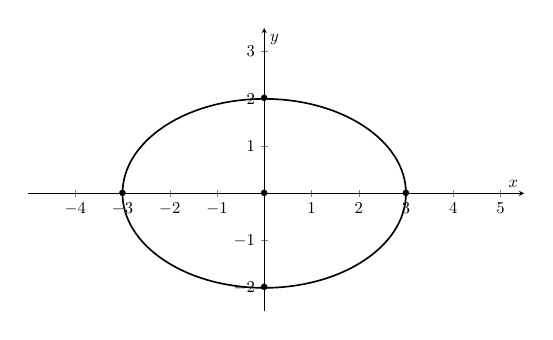
\begin{tikzpicture}[scale=0.6]
\begin{axis}[
x=1.0cm,y=1.0cm,
axis lines=middle,
xmin=-5,
xmax=5.5,
ymin=-2.5,
ymax=3.5,
xlabel=$x$, ylabel=$y$,
xtick={-4.0,-3.0,...,5.0},
ytick={-3.0,-2.0,...,3.0},]
\draw [rotate around={0.:(0.,0.)},line width=1pt] (0.,0.) ellipse (3.cm and 2.cm);
\draw(0,-2)node{$\bullet$};
\draw(0,2)node{$\bullet$};
\draw(-3,0)node{$\bullet$};
\draw(3,0)node{$\bullet$};
\draw(0,0)node{$\bullet$};
\end{axis}
\end{tikzpicture}
\end{center}
\end{enumerate}
\item   
\begin{enumerate}[k]
\item រកដែនកំណត់នៃអនុគមន៍$f$ 
\\ ដោយ $y=f(x)=\frac{x^2+3x-3}{x-1}$  \quad 
 គេបាន $f(x)$ មានន័យលុះត្រាតែ $x-1\neq 0\quad \Leftrightarrow\ x\neq 1$\\[0.2cm]
\textbf{ដូចនេះ}\  \fbox{ដែនកំនត់នៃអនុគមន៍ $f$ គឺ $D_f=\mathbb{R}-\{1\}$ }
\item គណនា $\lim_{x\to \pm \infty}f(x);\ \lim_{x\to 1}f(x)$
\begin{flalign*}
\lim_{x\to \pm \infty}f(x)&=\lim_{x\to\pm\infty}\frac{x^2+3x-3}{x-1}=\lim_{x\to \pm\infty}\frac{x^2}{x}=\pm\infty\quad \textbf{ដូចនេះ\ \fbox{$\lim_{x\to\pm \infty}f(x)=\pm\infty$}}&\\
\lim_{x\to 1}f(x) \ \ &=\lim_{x\to 1}\frac{x^2+3x-3}{x-1}=\pm \infty\quad \quad \quad\quad \quad \quad \ \ \textbf{ដូចនេះ}\ \fbox{$\lim_{x\to 1}f(x)=\pm\infty$}
\end{flalign*}
\item រកសមីការអាស៊ីមតូតឈរ និង សមីការអាស៊ីមតូតទ្រេត
\begin{itemize}
\item ដោយ $\lim_{x\to 1}f(x)=\pm\infty$\quad \textbf{ដូចនេះ}\ \fbox{ បន្ទាត់ $x=1$ ជាសមីការអាស៊ីមតូតឈរ}
\item ដោយ $y=f(x)=\frac{x^2+3x-3}{x-1}=x+4+\frac{1}{x-1}$\quad  គេបាន $\lim_{x\to \pm\infty}\frac{1}{x-1}=0$\\[0.2cm]
\textbf{ដូចនេះ} \ \fbox{បន្ទាត់ $y=x+4$ ជាសមីការអាស៊ីមតូតទ្រេត}
\end{itemize}
\item គណនាដេរីវេ $f'(x)$ និង សិក្សាសញ្ញាដេរីវេ $f'(x)$ 
\begin{flalign*}
f'(x)&=\left(\frac{x^2+3x-3}{x-1}\right)'=\frac{\left(x^2+3x-3\right)'(x-1)-(x-1)'\left(x^2+3x-3\right)}{(x-1)^2}=\frac{(2x+3)(x-1)-\left(x^2+3x-3\right)}{(x-1)^2}&\\
&=\frac{2x^2-2x+3x-3-x^2-3x+3}{(x-1)^2}=\frac{x^2-2x}{(x-1)^2}\\
f'(x)&=0\quad\Leftrightarrow\ x^2-2x=0\quad \Leftrightarrow x(x-2)=0\quad\Rightarrow\ \left[\begin{array}{l}
x=0\\
x-2=0\quad\Rightarrow \ x=2
\end{array}\right.
\end{flalign*}
 តារាសញ្ញាដេរីវេ $f'(x)$
\\[0.2cm]
\begin{tikzpicture}[scale=0.5]
   \tkzTabInit{$x$ / 1.5 , $f'(x)$ / 2}{$\ \ -\infty$ , $0$,$1$,$2$, $+\infty\ \ $}
   \tkzTabLine{, +, z, - ,d,-, z,+ }
\end{tikzpicture}\\
 បរមាធៀប 
\begin{itemize}
\item ត្រង់ $x=0;\ f'(x)=0$ ប្តូរសញ្ញាពី $+$ ទៅ $-$ គេបាន $f$ មានអតិបរមាធៀបមួយ គឺ $f(0)=\frac{0^2+3(0)-3}{0-1}=3$
\item ត្រង់ $x=2;\ f'(x)=0$ ប្តូរសញ្ញាពី $-$ ទៅ $+$ គេបាន $f$ មានអប្បបរមាធៀបមួយ គឺ $f(2)=\frac{2^2+3(2)-3}{2-1}=7$
\end{itemize}
\item សង់តារាងអថេរភាព និង សង់ក្រាប$(C)$ 
\begin{itemize}[2]
\item តារាងអថេរភាពនៃ $f$\\[0.2cm]
\begin{tikzpicture}[scale=0.5]
\begin{scriptsize}
   \tkzTabInit{$x$ / 1 , $f'(x)$ / 1.25, $f(x)$/3}{$\ \ -\infty$ , $0$,$1$,$2$, $+\infty\ \ $}
   \tkzTabLine{, +, z, - ,d,-, z,+ }
   \tkzTabVar{-/ $\ \ \ \  -\infty$, +/$3$, -D+/ $-\infty$ /$+\infty$, -/ $7$ , +/ $+\infty\ \ \ \ $}
\end{scriptsize}
\end{tikzpicture}
{}\\{}\\{}\\{}\\{}\\{}\\{}
\item ក្រាប $C$  
\begin{center}
\definecolor{qqwuqq}{rgb}{0.,0.39215686274509803,0.}
\begin{tikzpicture}[scale=0.6]
\begin{scriptsize}[scale=0.5]
\draw(0,9)node{$
\begin{array}{l}
(d):\ y=x+4\\
\begin{tabular}{c|cc}
$x$&$0$&$-4$\\
\hline 
$y$&$4$&$0$
\end{tabular}
\end{array}
$};
\end{scriptsize}
\begin{axis}[
x=1.0cm,y=1.0cm,
axis lines=middle,
xmin=-5,
xmax=7,
ymin=-2,
ymax=10,
xlabel=$x$,ylabel=$y$,
xtick={-4,-3.0,-2.0,...,6.0},
ytick={-2.0,-1.0,...,7,8,9}]
\draw[line width=1.pt,color=qqwuqq,smooth,samples=90,domain=-5:5.8] plot(\x,{((\x)^(2)+3*(\x)-3)/((\x)-1.0)});
\draw [line width=1.pt,domain=-5.:6.] plot(\x,{\x+4});
\draw(3,6)node[right=-0.5cm]{$(d):\ y=x+4$};
\draw(1.75,9)node[color=qqwuqq]{$(c)$};
\draw(1.5,-1.5)node[color=qqwuqq]{$x=1$};
\draw [dashed](2,0)--(2,7)node{$\bullet$}--(0,7); 
\draw [dashed](0,0)--(0,3)node{$\bullet$}--(0,3); 
\end{axis}
\end{tikzpicture}
\end{center}
\end{itemize}
\end{enumerate}
\end{enumerate}	

\newpage 
\maketitle 
    \borderline{វិញ្ញាសាទី៧}
\begin{enumerate}[I]
\item (១០ពិន្ទុ) ចូរគណនាតម្លៃនៃលីមីតខាងក្រោម៖
\begin{enumerate}[k,3]
\item $\lim_{x\to 1}\frac{x^2-1}{\sqrt{x}-1}$ 
\item $\lim_{x\to 2}\frac{x^3-8}{\sqrt{x+2}-2}$
\item $\lim_{x\to 1}\frac{x^2+4x-5}{x-1}$
\end{enumerate}
\item (១០ពិន្ទុ) ក្នុងថង់មួយមានប៊ូលខៀវចំនួន $3$ និងប៊ូលពណ៌ខ្មៅចំនួន $5$។ គេចាប់យកប៊ូល $2$ ចេញពីថង់ដោយចៃដន្យ។ ចូររកប្រូបាបនៃព្រឹត្តិការណ៍ខាងក្រោម៖
\begin{enumerate}[k]
\item « គេចាប់បានប៊ូលពណ៌ខៀវទាំងអស់ »
\item «គេចាប់បានប៊ូលពណ៌ខ្មៅទាំងអស់»
\item «គេចាប់បានប៊ូលមួយក្នុងមួយពណ៌»
\end{enumerate}
\item (១០ពិន្ទុ)  ចូរគណនាអាំងតេក្រាលខាងក្រោម៖
\begin{enumerate}[k,3]
\item $\mathrm{I}=\int_1^3x^2dx$
\item $\mathrm{J}=\int_1^4\left(2x^2-4x+4\right)dx$
\item $\mathrm{K}=\int_1^3\left(x^2+\frac{1}{x}-e^x\right)dx$
\end{enumerate}
\item (១៥ពិន្ទុ) គេមានសមីការ $16x^2+9y^2=144$ ។
\begin{enumerate}[k]
\item បង្ហាញថាសមីការនេះជាសមីការអេលីប។
\item ចូររកប្រវែងអ័ក្សធំ ប្រវែងអ័ក្សតូច កូអរដោនេនៃកំពូលទាំងពីរ និងកូអរដោនេនៃកំណុំទាំងពីរ។
\item ចូរសង់អេលីប។
\end{enumerate}
\item (៣០ពិន្ទុ) អនុគមន៍ $f$ កំណត់ដោយ $y=f(x)=\frac{x^2-3x-3}{x-2}$ មានក្រាបតំណាង $(C)$ ។
\begin{enumerate}[k]
\item ចូររកដែនកំណត់នៃអនុគមន៍ $f$ ។
\item ចូរគណនា $\lim_{x\to 2}f(x);\ \lim_{x\to -\infty}f(x);\ \lim_{x\to +\infty}f(x)$។ រួចទាញរកសមីការអាស៊ីមតូតឈរនៃក្រាប $(C)$ ។
\item ចូរបង្ហាញថា $f(x)=x-1+\frac{-5}{x-2}$ ។ រួចទាញរកសមីការអាស៊ីមតូតទ្រេត។
\item សិក្សាអថេរភាព សង់តារាងអថេរភាព និង សង់ក្រាប$(C)$។ 
\end{enumerate}
\end{enumerate}
\newpage 
\borderline{ចម្លើយ}
\begin{enumerate}[I]
\item គណនាតម្លៃនៃលីមីត៖
\begin{enumerate}[k]
\item $\lim_{x\to 1}\frac{x^2-1}{\sqrt{x}-1}$ \quad (មានរាងមិនកំណត់$\tfrac{0}{0}$)
\begin{flalign*}
&=\lim_{x\to 1}\frac{\left(x^2-1\right)\left(\sqrt{x}+1\right)}{\left(\sqrt{x}-1\right)\left(\sqrt{x}+1\right)}=\lim_{x\to 1}\frac{(x-1)(x+1)\left(\sqrt{x}+1\right)}{x-1}=\lim_{x\to 1} {(x+1)\left(\sqrt{x}+1\right)}= {(1+1)\left(\sqrt{1}+1\right)}=4&
\end{flalign*}
ដូចនេះ \ \fbox{$\lim_{x\to 1}\frac{x^2-1}{\sqrt{x}-1}=4$}
\item $\lim_{x\to 2}\frac{x^3-8}{\sqrt{x+2}-2}$\quad (មានរាងមិនកំណត់$\tfrac{0}{0}$)
\begin{flalign*}
&=\lim_{x\to 2}\frac{\left(x^3-2^3\right)\left(\sqrt{x+2}+2\right)}{\left(\sqrt{x+2}-2\right)\left(\sqrt{x+2}+2\right)}=\lim_{x\to 2}\frac{(x-2)\left(x^2+2x+2^2\right)\left(\sqrt{x+2}+2\right)}{x+2-2^2}&\\
&=\lim_{x\to 2}\frac{(x-2)\left(x^2+2x+4\right)\left(\sqrt{x+2}+2\right)}{x-2}=\lim_{x\to 2}\left(x^2+2x+4\right)\left(\sqrt{x+2}+2\right)=\left(2^2+2(2)+4\right)\left(\sqrt{2+2}+2\right)\\
&=12(4)=48
\end{flalign*}
ដូចនេះ\ \fbox{$\lim_{x\to 2}\frac{x^3-8}{\sqrt{x+2}-2}=48$}
\item $\lim_{x\to 1}\frac{x^2+4x-5}{x-1}$\quad (មានរាងមិនកំណត់$\tfrac{0}{0}$)
\begin{flalign*}
&=\lim_{x\to 1}\frac{(x-1)(x+5)}{x-1}=\lim_{x\to 1}(x+5)=1+5=6\quad\quad\textbf{ដូចនេះ}\ \fbox{$\lim_{x\to 1}\frac{x^2+4x-5}{x-1}=6$}&
\end{flalign*}
\end{enumerate}
\item  រកប្រូបាបនៃព្រឹត្តិការណ៍៖
\begin{enumerate}[k]
\item « គេចាប់បានប៊ូលពណ៌ខៀវទាំងអស់ »\quad\quad តាង \ $\mathrm{A}:$ « គេចាប់បានប៊ូលពណ៌ខៀវទាំងអស់ »
\begin{flalign*}
\textbf{តាមរូបមន្ត}\ P(A)=\frac{n(A)}{n(S)}\quad \text{ដោយ}\ &n(A)=C(3,2)=\frac{3!}{(3-2)!2!}=\frac{3\times 2!}{1!2!}=\frac{3}{1}=3&\\
&n(S)=C(8,2)=\frac{8!}{6!2!}=\frac{8\times 7\times 6!}{6!\times 2\times 1}=28 
\end{flalign*}
គេបាន $P(A)=\frac{n(A)}{n(S)}=\frac{3}{28}$\quad ដូចនេះ\ \fbox{$P(A)=\frac{3}{28}$}
\item «គេចាប់បានប៊ូលពណ៌ខ្មៅទាំងអស់» \quad\quad តាង \ $\mathrm{B}:$ « គេចាប់បានប៊ូលពណ៌ខ្មៅទាំងអស់ »
\begin{flalign*}
\textbf{តាមរូបមន្ត}\ P(B)=\frac{n(B)}{n(S)}\quad \text{ដោយ}\ &n(B)=C(5,2)=\frac{5!}{(5-2)!2!}=\frac{5\times 4\times 3!}{3!2\times 1}=10;\quad
 n(S)=28  &
\end{flalign*}
គេបាន $P(B)=\frac{n(B)}{n(S)}=\frac{10}{28}=\frac{5}{14}$\quad ដូចនេះ\ \fbox{$P(B)=\frac{5}{14}$}
\item «គេចាប់បានប៊ូលមួយក្នុងមួយពណ៌» \quad\quad តាង \ $\mathrm{C}:$ « គេចាប់បានប៊ូលមួយក្នុងមួយពណ៌ »
\begin{flalign*}
\textbf{តាមរូបមន្ត}\ P(C)=\frac{n(C)}{n(S)}\quad \text{ដោយ}\ &n(C)=C(3,1)\times C(5,1)=\frac{3!}{2!1!}\times \frac{5!}{4!1!}=\frac{3\times 2!}{2!}\times\frac{5\times 4!}{4!}=3\times 5=15&\\
&n(S)=28 
\end{flalign*}
គេបាន $P(C)=\frac{n(C)}{n(S)}=\frac{15}{28}$
\quad ដូចនេះ\ \fbox{$P(C)=\frac{15}{28}$}
\end{enumerate}

\item គណនាអាំងតេក្រាល៖
\begin{enumerate}[k]
\item $\mathrm{I}=\int_1^3x^2dx=\left[\frac{x^3}{3}\right]_1^3=\frac{3^3}{3}-\frac{1^3}{3}=\frac{27-1}{3}=\frac{26}{3}$\quad\quad ដូចនេះ\ \fbox{$\int_1^3x^2dx=\frac{26}{3}$}
\item $\mathrm{J}=\int_1^4\left(2x^2-4x+4\right)dx=\left[\frac{2x^3}{3}-\frac{4x^2}{2}+4x\right]_1^4=\frac{2(4)^3}{3}-2(4)^2+4(4)-\left(\frac{2(1)^3}{3}-2(1)^2+4(1)\right)$
\begin{flalign*}
&\ =\frac{128}{3}-16-\frac{2}{3}-2 =\frac{126}{3}-18=\frac{126-54}{3}=\frac{72}{3}=24\quad\text{ដូចនេះ} \ \fbox{$\mathrm{J}=24$}&
\end{flalign*}
\item $\mathrm{K}=\int_1^3\left(x^2+\frac{1}{x}-e^x\right)dx=\left[\frac{x^3}{3}+\ln |x|-e^x\right]_1^3=\frac{3^3}{3}+\ln 3-e^3-\left(\frac{1^3}{3}+\ln 1-e^1\right)=\frac{27}{3}+\ln 3-e^3-\frac{1}{3}-0+e$
\begin{flalign*}
&\ \ =\frac{26}{3}+\ln 3-e^3+e\quad \text{ដូចនេះ} \ \fbox{$\mathrm{K}=\frac{26}{3}+\ln 3-e^3+e$}&
\end{flalign*}
\end{enumerate}
\item  
\begin{enumerate}[k]
\item បង្ហាញថាសមីការ $16x^2+9y^2=144$ ជាសមីការអេលីប
\begin{flalign*}
16x^2+9y^2=144\quad \Leftrightarrow\ & \frac{16x^2}{144}+\frac{9y^2}{144}=\frac{144}{144}&\\
\Leftrightarrow\ &\frac{x^2}{9}+\frac{y^2}{16}=1\\
\Leftrightarrow\ &\frac{(x-0)^2}{3^2}+\frac{(y-0)^2}{4^2}=1\quad\quad\textbf{ជាសមីការអេលីប ដែលមានផ្ចិត} (0,0)
\end{flalign*}
ដូចនេះ\ \fbox{ សមីការ $16x^2+9y^2=144$ ជាសមីការអេលីប }
\item ប្រវែងអ័ក្សធំ ប្រវែងអ័ក្សតូច កូអរដោនេនៃកំពូលទាំងពីរ និងកូអរដោនេនៃកំណុំទាំងពីរ
\\ ដោយ អេលីបមានសមីការ $\frac{(x-0)^2}{3^2}+\frac{(y-0)^2}{4^2}=1$ គេបាន
\begin{itemize}[p]
\item $h=0\ ;\ k=0;\quad\quad\quad a=4;\ b=3;\quad\quad\quad c^2=a^2-b^2=16-9=7\quad\Rightarrow\ c=\sqrt{7}$
\item អ័ក្សធំជាអ័ក្សឈរ
\begin{itemize}
\item ប្រវែងអ័ក្សធំ $=2a=2(4)=8$
\item ប្រវែងអ័ក្សតូច $=2b=2(3)=6$
\item កំពូល $V_1(h,k-a);\ V_2(h,k+a)\quad \Rightarrow\ V_1(0,-4);\ V_2(0,3)$
\item កំណុំ $F_1(h,k-c);\ F_2(h,k+c)\quad\Rightarrow\ F_1(0,-\sqrt{7});\ F_2(0,\sqrt{7})$
\end{itemize}
\end{itemize}
\item សង់អេលីប
\begin{center}
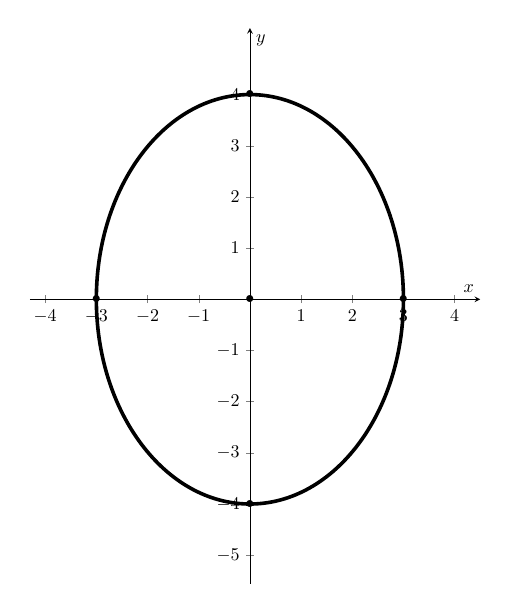
\begin{tikzpicture}[scale=0.65]
\begin{axis}[
x=1.0cm,y=1.0cm,
axis lines=middle,
xmin=-4.3,
xmax=4.5,
ymin=-5.56,
ymax=5.3, xlabel=$x$,ylabel=$y$,
xtick={-4.0,-3.0,...,4.0},
ytick={-5,-4,-3,-2.0,-1.0,...,4.0},]
\draw [rotate around={90.:(0.,0.)},line width=2.pt] (0.,0.) ellipse (4.cm and 3.cm);
\draw(0,4)node{$\bullet$};
\draw(0,-4)node{$\bullet$};
\draw(3,0)node{$\bullet$};
\draw(-3,0)node{$\bullet$};
\draw(0,0)node{$\bullet$};
\end{axis}
\end{tikzpicture}
\end{center}
\end{enumerate}
\item
\begin{enumerate}[k]
\item រកដែនកំណត់នៃអនុគមន៍ $f$ \\
ដោយ $y=f(x)=\frac{x^2-3x-3}{x-2}$ \quad ដោយ \ $f(x)$ មានន័យលុះត្រាតែ $x-2\neq 0\quad\Leftrightarrow\ x\neq 2$\\[0.2cm]
ដូចនេះ\ \fbox{$D_f=\mathbb{R}-\{2\}$}
\item គណនា $\lim_{x\to 2}f(x);\ \lim_{x\to -\infty}f(x);\ \lim_{x\to +\infty}f(x)$។ រួចទាញរកសមីការអាស៊ីមតូតឈរនៃក្រាប $(C)$ 
\begin{flalign*}
&\lim_{x\to 2}f(x)\ \ =\lim_{x\to 2}\ \frac{x^2-3x-3}{x-2}=\pm \infty\quad \quad\quad\quad\quad \quad\ \  \textbf{ដូចនេះ}\ \fbox{$\lim_{x\to 2}f(x)=\pm\infty$} &\\
&\lim_{x\to -\infty}f(x)=\lim_{x\to -\infty}\frac{x^2-3x-3}{x-2}=\lim_{x\to -\infty}\frac{x^2}{x}=-\infty\quad \textbf{ដូចនេះ}\ \fbox{$\lim_{x\to -\infty}f(x)=-\infty$}\\
&\lim_{x\to +\infty}f(x)=\lim_{x\to +\infty}\frac{x^2-3x-3}{x-2}=\lim_{x\to +\infty}\frac{x^2}{x}=+\infty\quad \textbf{ដូចនេះ}\ \fbox{$\lim_{x\to +\infty}f(x)=+\infty$}
\end{flalign*}
ដោយ $\lim_{x\to 2}f(x)=\pm\infty$ ដូចនេះ\ \fbox{បន្ទាត់ $x=2$ ជាអាស៊ីមតូតឈរ}
\item បង្ហាញថា $f(x)=x-1+\frac{-5}{x-2}$  រួចទាញរកសមីការអាស៊ីមតូតទ្រេត
\begin{flalign*}
\text{ដោយ}\ x-1+\frac{-5}{x-2}&=\frac{(x-1)(x-2)-5}{x-2}=\frac{x^2-2x-x+2-5}{x-2}=\frac{x^2-3x-3}{x-2}=f(x)&
\end{flalign*}
ដូចនេះ\ \fbox{$f(x)=x-1+\frac{-5}{x-2}$}\quad ដោយ\ $\lim_{x\to \pm\infty}\frac{-5}{x-2}=0$\quad ដូចនេះ\ \fbox{បន្ទាត់ $y=x-1$ ជាអាស៊ីមតូតទ្រេត }
\item សិក្សាអថេរភាព សង់តារាងអថេរភាព និង សង់ក្រាប$(C)$
\begin{flalign*}
f'(x)&=\left(\frac{x^2-3x-3}{x-2}\right)'=\frac{\left(x^2-3x-3\right)'(x-2)-(x-2)'\left(x^2-3x-3\right)}{(x-2)^2}&\\
&=\frac{(2x-3)(x-2)-\left(x^2-3x-3\right)}{(x-2)^2}=\frac{2x^2-4x-3x+6-x^2+3x+3}{(x-2)^2}=\frac{x^2-4x+9}{(x-2)^2}\\
f'(x)&=0\quad\Leftrightarrow\ x^2-4x+9=0 ; \ \ \Delta =b^2-4ac=16-4(1)(9)=-20<0\quad \Rightarrow \ f'(x) \text{មានសញ្ញាតាមមេគុណ } a 
\end{flalign*}
\begin{itemize}[2]
\item តារាងសញ្ញា $f'(x)$		
\\[0.2cm]
\begin{tikzpicture}[scale=0.5]
   \tkzTabInit{$x$ / 1.5 , $f'(x)$ / 2}{$\ \ -\infty$ , $2$, $+\infty\ \ $}
   \tkzTabLine{,+,d,+, }
\end{tikzpicture}	
\item តារាងអថេរភាពនៃ $f$
\\[0.2cm]
\begin{tikzpicture}[scale=0.8]
   \tkzTabInit{$x$ / 1 , $f'(x)$ / 1.25, $f(x)$/2}{$\ \ -\infty$ ,$2$, $+\infty\ \ $}
   \tkzTabLine{, +, d, + , }
   \tkzTabVar{-/ $-\infty$,  +D-/ $+\infty$ /$-\infty$, +/ $+\infty$ }
\end{tikzpicture}
{}\\{}\\{}\\{}\\{}\\{}\\{}
\item សង់ក្រាប $(C)$
\begin{itemize}
\item $C\cap (y'oy)$ គឺ $x=0\Rightarrow\ y=\tfrac{3}{2}$
\item  $C\cap (x'ox)$ គឺ $y=0\Rightarrow\ x=\tfrac{3\pm\sqrt{21}}{2} $
\end{itemize}
\begin{center}
\definecolor{qqwuqq}{rgb}{0.,0.39215686274509803,0.}
\begin{tikzpicture}[scale=0.5]
\begin{scriptsize}[scale=0.5]
\draw(5,15)node{$
\begin{array}{l}
(d):\ y=x-1\\
\begin{tabular}{c|cc}
$x$&$0$&$1$\\
\hline 
$y$&$-1$&$0$
\end{tabular}
\end{array}
$};
\end{scriptsize}
\begin{axis}[
x=1.0cm,y=1.0cm,
axis lines=middle,
xmin=-8.5,
xmax=8.2,
ymin=-9,
ymax=8.5,
xlabel=$x$,ylabel=$y$,
xtick={-8,-7,-6.0,-5.0,...,6.0,7,8},
ytick={-8,-7,-6.0,-5.0,...,7.0},]
\draw[line width=1.pt,color=qqwuqq,smooth,samples=80,domain=-8:8] plot(\x,{((\x)^(2)-3*(\x)-3)/((\x)-2)});
\draw [line width=1.pt,domain=-8.:8] plot(\x,{\x-1});
\draw(7,7)node{$(d):\ y=x-1$};
\draw(1,7)node[color=qqwuqq]{$(c)$};
\draw(1.6,-8)node[color=qqwuqq]{$x=2$};
\draw [dashed](2,0)--(2,1)node{$\bullet$}--(0,1); 
\end{axis}
\end{tikzpicture}
\end{center}
\end{itemize}
\end{enumerate}
\end{enumerate}

\newpage 
\maketitle 
    \borderline{វិញ្ញាសាទី៨}
\begin{enumerate}[I]
\item (១៥ពិន្ទុ) ក្នុងប្រអប់ប៊ិចមួយមានប៊ិចពណ៌ខៀវ $5$ ដើម និងប៊ិចពណ៌ក្រហម $6$ ដើម។ គេបានដកយកប៊ិច $4$ ដើមចេញមកក្រៅដោយចៃដន្យ។  ចូររកប្រូបាបនៃព្រឹត្តិការណ៍ខាងក្រោម៖
\begin{enumerate}[A]
\item : «គេចាប់បានប៊ិចពណ៌ខៀវទាំង $4$ ដើម»
\item : «គេចាប់បានប៊ិចពណ៌ខៀវ $2$ ដើម និង ប៊ិចពណ៌ក្រហម $2$ ដើម»
\item : «គេចាប់បានប៊ិចក្រហមយ៉ាងតិច $1$ ដើម»
\end{enumerate}
\item (១០ពិន្ទុ) ចូរគណនាតម្លៃនៃលីមីតខាងក្រោម៖
\begin{enumerate}[k,3]
\item $\lim_{x\to 1}\frac{x^3-1}{x^2-1}$ 
\item $\lim_{x\to 0}\frac{x^2-2x}{\sqrt{9+x}-3}$
\item $\lim_{x\to 1}\frac{x^2+4x-5}{x^2-2x+1}$
\end{enumerate}
\item (១០ពិន្ទុ) 
\begin{enumerate}[k]
\item គណនា $\mathrm{I}=\int_0^1\left(1+\frac{1}{x}+\frac{1}{x^2}\right)dx$ ។
\item គេមាន $f(x)=\frac{x^2-5x+5}{1-x}$។ ចូរបង្ហាញថា $f(x)=-x+4+\frac{1}{1-x}$។ រួចគណនា $\mathrm{K}=\int_0^2 f(x)dx$។
\end{enumerate}
\item (១០ពិន្ទុ) គេមានសមីការអេលីប $25x^2+4y^2=100$ ។
\begin{enumerate}[k]
\item ចូរសរសេរសមីការស្តង់ដានៃអេលីបនេះ រួចទាញរកកូអរដោនេនៃកំពូលទាំងពីរ និងកូអរដោនេនៃកំណុំទាំងពីរ។
\item ចូររកប្រវែងអ័ក្សធំ និង ប្រវែងអ័ក្សតូច រួចសង់អេលីបនេះ។
\end{enumerate}
\item (៣០ពិន្ទុ) គេអោយអនុគមន៍ $f$ កំណត់ដោយ $f(x)=\frac{x^2-5x+7}{x-2}$ មានក្រាបតំណាង $(C)$ ។
\begin{enumerate}[k]
\item រកដែនកំណត់នៃអនុគមន៍ $f$ ។ 
\item គណនា $\lim_{x\to 2}f(x);\ \lim_{x\to\pm\infty}f(x)$។ ទាញរកសមីការអាស៊ីមតូតឈរនៃក្រាប $C$ ។
\item រកតម្លៃនៃចំនួនពិត $a,b$ និង $c$ ដែលធ្វើអោយ $f(x)=ax+b+\frac{c}{x-2}$។ បង្ហាញថា បន្ទាត់ $d$ ដែលមានសមីការ $y=x-3+\frac{1}{x-2}$ ជាអាស៊ីមតូតទ្រេតនៃក្រាប $C$ ត្រង់ $\pm\infty$ ។
\item សិក្សាអថេរភាព និងសង់ក្រាប $C$។
\end{enumerate}
\end{enumerate}
\newpage 
\borderline{ចម្លើយ}
\begin{enumerate}[I]
\item  រកប្រូបាបនៃព្រឹត្តិការណ៍ខាងក្រោម៖
\begin{enumerate}[A]
\item : «គេចាប់បានប៊ិចពណ៌ខៀវទាំង $4$ ដើម»
\begin{flalign*}
\textbf{តាមរូបមន្ត}\ P(A)=\frac{n(A)}{n(S)}\quad \text{ដោយ}\ &n(A)=C(5,4)=\frac{5!}{(5-4)!4!}=\frac{5\times 4!}{1!4!}=5&\\
&n(S)=C(11,4)=\frac{11!}{(11-4)!4!}=\frac{11\times 10\times 9\times 8\times 7!}{7!\times 4\times 3\times 2\times 1}=330
\end{flalign*}
គេបាន  \ $P(A)=\frac{n(A)}{n(S)}=\frac{5}{330}=\frac{1}{66}$\quad ដូចនេះ\ \fbox{$P(A)=\frac{1}{66}$}
\item : «គេចាប់បានប៊ិចពណ៌ខៀវ $2$ ដើម និង ប៊ិចពណ៌ក្រហម $2$ ដើម»
\begin{flalign*}
\textbf{តាមរូបមន្ត}\ P(B)=\frac{n(B)}{n(S)}\quad \text{ដោយ}\ &n(B)=C(5,2)\times C(6,2)=\frac{5!}{3!2!}\times\frac{6!}{4!2!}=\frac{5\times 4\times 3!}{3!\times 2\times 1}\times\frac{6\times 5\times 4!}{4!\times 2\times 1}=150& 
\end{flalign*}
គេបាន  \ $P(B)=\frac{n(B)}{n(S)}=\frac{150}{330}=\frac{5}{11}$\quad ដូចនេះ\ \fbox{$P(B)=\frac{5}{11}$}
\item : «គេចាប់បានប៊ិចក្រហមយ៉ាងតិច $1$ ដើម»
\begin{flalign*}
\textbf{តាមរូបមន្ត} \ P(C)&=1-P(A) \quad \text{ដោយ}\ P(A)=\frac{1}{66}&\\
\Rightarrow\quad P(C)&=1-\frac{1}{66}=\frac{66-1}{66}=\frac{65}{66}\quad\quad\textbf{ដូចនេះ}\ \fbox{$P(C)=\frac{65}{66}$}
\end{flalign*}
\end{enumerate}
\item គណនាលីមីត
\begin{enumerate}[k]
\item $\lim_{x\to 1}\frac{x^3-1}{x^2-1}$ \quad (មានរាងមិនកំណត់$\tfrac{0}{0}$)
\begin{flalign*}
&=\lim_{x\to 1}\frac{(x-1)\left(x^2+x+1\right)}{(x-1)(x+1)}=\lim_{x\to 1}\frac{x^2+x+1}{x+1}=\frac{1^2+1+1}{1+1}=\frac{3}{2} \quad \text{ដូចនេះ} \ \fbox{$\lim_{x\to 1}\frac{x^3-1}{x^2-1}=\frac{3}{2}$}&
\end{flalign*}

\item $\lim_{x\to 0}\frac{x^2-2x}{\sqrt{9+x}-3}$\quad (មានរាងមិនកំណត់$\tfrac{0}{0}$)
\begin{flalign*}
&=\lim_{x\to 0}\frac{\left(x^2-2x\right)\left(\sqrt{9+x}+3\right)}{\left(\sqrt{9+x}-3\right)\left(\sqrt{9+x}+3\right)}=\lim_{x\to 0}\frac{x(x-2)\left(\sqrt{9+x}+3\right)}{9+x-9}=\lim_{x\to 0}(x-2)\left(\sqrt{9+x}+3\right)&\\
& =(0-2)\left(\sqrt{9+0}+3\right)=-2(6)=-12\quad \quad \textbf{ដូចនេះ}\ \fbox{$\lim_{x\to 0}\frac{x^2-2x}{\sqrt{9+x}-3}=-12$}&
\end{flalign*}
\item $\lim_{x\to 1}\frac{x^2+4x-5}{x^2-2x+1}$\quad (មានរាងមិនកំណត់$\tfrac{0}{0}$)
\begin{flalign*}
&=\lim_{x\to 1}\frac{(x-1)(x+5)}{(x-1)(x-1)}=\lim_{x\to 1}\frac{x+5}{x-1}=\pm\infty\quad\quad\textbf{ដូចនេះ}\ \fbox{$\lim_{x\to 1}\frac{x^2+4x-5}{x^2-2x+1}=\pm\infty$}&
\end{flalign*}
\end{enumerate}
\item 
\begin{enumerate}[k]
\item គណនា $\mathrm{I}$ 
\begin{flalign*}
\mathrm{I}&=\int_1^e\left(1+\frac{1}{x}+\frac{1}{x^2}\right)dx=\left[x+\ln |x|-\frac{1}{x}\right]_1^e=e+\ln e-\frac{1}{e}-\left(1+\ln 1 -\frac{1}{1} \right)=e+1-\frac{1}{e}-1-0+1=e+1-\frac{1}{e}&
\end{flalign*}
ដូចនេះ \ \fbox{$\mathrm{I}=e+1-\frac{1}{e}$}
\item គេមាន $f(x)=\frac{x^2-5x+5}{1-x}$ បង្ហាញថា $f(x)=-x+4+\frac{1}{1-x}$
\begin{flalign*}
\textbf{ដោយ}\ -x+4+\frac{1}{1-x}&=\frac{(-x+4)(1-x)+1}{1-x}=\frac{-x+x^2+4-4x+1}{1-x}=\frac{x^2-5x+5}{1-x}=f(x)&
\end{flalign*}
ដូចនេះ\ \fbox{$f(x)=-x+4+\frac{1}{1-x}$}
\\[0.2cm]
 គណនា $\mathrm{K}$
 \begin{flalign*}
 \mathrm{K}&=\int_0^2f(x)dx=\int_0^2 \left(-x+4+\frac{1}{1-x}\right)dx=\left[-\frac{x^2}{2}+4x-\ln |1-x|\right]_0^2&\\
 &=-\frac{2^2}{2}+4(2)-\ln |1-2|-\left(-\frac{0^2}{2}+4(0)-\ln 1\right)=-2+8-0+0+0-0=6\quad \text{ ដូចនេះ} \ \fbox{$\mathrm{K}=6$}
 \end{flalign*}
\end{enumerate}

\item (១០ពិន្ទុ) គេមានសមីការអេលីប ។
\begin{enumerate}[k]
\item សរសេរសមីការស្តង់ដានៃអេលីប  $25x^2+4y^2=100$
\begin{flalign*}
 25x^2+4y^2=100\quad\Leftrightarrow\ & \frac{25x^2}{100}+\frac{4y^2}{100}=\frac{100}{100}&\\
 \Leftrightarrow\ &\frac{x^2}{4}+\frac{y^2}{25}=1\\
 \Leftrightarrow\ &\frac{(x-0)^2}{2^2}+\frac{(y-0)^2}{5^2}=1 \quad \textbf{ជាសមីការស្តង់ដានៃអេលីប ដែលមានផ្ចិត} (0,0)
\end{flalign*}

ទាញរកកូអរដោនេនៃកំពូលទាំងពីរ និងកូអរដោនេនៃកំណុំទាំងពីរ
\\
ដោយ សមីការស្តង់ដានៃអេលីបគឺ $\frac{(x-0)^2}{2^2}+\frac{(y-0)^2}{5^2}=1$ គេបាន
\begin{itemize}[p]
\item អ័ក្សធំជាអ័ក្សឈរ
\item $h=0,\ k=0\quad\quad , a=5,\ b=2,\quad \quad c^2=a^2-b^2=25-4=21\quad\Rightarrow \ c=\sqrt{21}$
\begin{itemize}
\item កំពូល $V_1(h,k-a);\ V_2(h,k+a)\quad\Rightarrow\ V_1(0,-5),\ V_2(0,5)$
\item កំណុំ $F_1(h,k-c);\ F_2(h,k+c)\quad\Rightarrow\ F_1(0,-\sqrt{21});\ F_2(0,\sqrt{21})$
\end{itemize}
\end{itemize}

\item រកប្រវែងអ័ក្សធំ  ប្រវែងអ័ក្សតូច និង សង់អេលីប
\begin{itemize}[2]
\item ប្រវែងអ័ក្សធំ $=2a=2(5)=10$
\item ប្រវែងអ័ក្សតូច $=2b=2(2)=4$
\item សង់អេលីប
\\
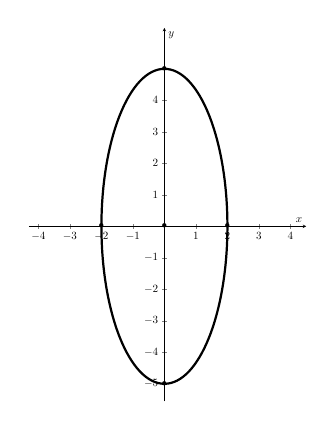
\begin{tikzpicture}[scale=0.4]
\begin{axis}[
x=1.0cm,y=1.0cm,
axis lines=middle,
xmin=-4.3,
xmax=4.5,
ymin=-5.56,
ymax=6.3, xlabel=$x$,ylabel=$y$,
xtick={-4.0,-3.0,...,4.0},
ytick={-5,-4,-3,-2.0,-1.0,...,4.0},]
\draw [rotate around={90.:(0.,0.)},line width=2.pt] (0.,0.) ellipse (5.cm and 2.cm);
\draw(0,5)node{$\bullet$};
\draw(0,-5)node{$\bullet$};
\draw(2,0)node{$\bullet$};
\draw(-2,0)node{$\bullet$};
\draw(0,0)node{$\bullet$};
\end{axis}
\end{tikzpicture}

\end{itemize}
\end{enumerate}

\item 
\begin{enumerate}[k]
\item រកដែនកំណត់នៃអនុគមន៍ $f$  \\
ដោយ $f(x)=\frac{x^2-5x+7}{x-2}$\quad $f(x)$ មានន័យលុះត្រាតែ $x-2\neq 0\quad\Leftrightarrow\ x\neq 2$\\
ដូចនេះ\ \fbox{ដែនកំណត់នៃអនុគមន៍ $f$ គឺ $D_f=\mathbb{R}-\{2\}$ } 
\item 
\begin{itemize}
\item គណនា $\lim_{x\to 2}f(x);\ \lim_{x\to\pm\infty}f(x)$
\begin{flalign*}
&\lim_{x\to 2}f(x)=\lim_{x\to 2}\frac{x^2-5x+7}{x-2}=\pm\infty\quad\quad  \textbf{ដូចនេះ}\ \fbox{$\lim_{x\to 2}f(x)=\pm\infty$}&\\
&\lim_{x\to \pm\infty}f(x)=\lim_{x\to \pm\infty}\frac{x^2-5x+7}{x-2}=\lim_{x\to \pm\infty}\frac{x^2}{x}=\pm\infty\quad\quad\textbf{ដូចនេះ}\ \fbox{$\lim_{x\to\pm\infty}f(x)=\pm\infty$}
\end{flalign*}
\item  ទាញរកសមីការអាស៊ីមតូតឈរនៃក្រាប $C$ 
 \\ ដោយ $\lim_{x\to 2}f(x)=\pm\infty$\quad  ដូចនេះ\ \fbox{បន្ទាត់ $x=2$ ជាសមីការអាស៊ីមតូតឈរ}
\end{itemize}
\item 
\begin{itemize}
\item រកតម្លៃនៃចំនួនពិត $a,b$ និង $c$ ដែលធ្វើអោយ $f(x)=ax+b+\frac{c}{x-2}$
\begin{flalign*}
f(x)=ax+b+\frac{c}{x-2}\quad \Leftrightarrow\ & \frac{x^2-5x+7}{x-2} =ax+b+\frac{c}{x-2}&\\
\Leftrightarrow \ &\frac{(x-3)(x-2)+1}{x-2}=ax+b+\frac{c}{x-2}\\
\Leftrightarrow\ & x-3+\frac{1}{x-2}=ax+b+\frac{c}{x-2}\quad\quad\quad \textbf{ផ្ទឹមមេគុណគេបាន}\  a=1,b=-3,c=1
\end{flalign*}
ដូចនេះ\ \fbox{$a=1,\ b=-3,\ c=1$}
\item 
 បង្ហាញថា បន្ទាត់ $d$ ដែលមានសមីការ $y=x-3$ ជាអាស៊ីមតូតទ្រេតនៃក្រាប $C$ ត្រង់ $\pm\infty$
 \begin{flalign*}
 &\text{យើងមាន}\ y=f(x)=x-3+\frac{1}{x-2}  \quad\text{ដោយ} \ \lim_{x\to \pm\infty}\frac{1}{x-2}=0&
 \end{flalign*}
 ដូចនេះ\ \fbox{បន្ទាត់ $d:\ y=x-3$ ជាអាស៊ីមតូតទ្រេតនៃក្រាប $C$ ត្រង់ $\pm\infty$}
\end{itemize} 
\item សិក្សាអថេរភាព និងសង់ក្រាប $C$
\begin{itemize}
\item ដេរីវេ 
\begin{flalign*}
f'(x)&=\left(\frac{x^2-5x+7}{x-2}\right)' =\frac{\left(x^2-5x+7\right)'(x-2)-(x-2)'\left(x^2-5x+7\right)}{(x-2)^2}&\\
&=\frac{(2x-5)(x-2)-\left(x^2-5x+7\right)}{(x-2)^2}=\frac{2x^2-4x-5x+10-x^2+5x-7}{(x-2)^2}=\frac{x^2-4x+3}{(x-2)^2}\\
f'(x)&=0\quad\Leftrightarrow\ x^2-4x+3=0 \quad \text{មានឫស}\  x_1=1;\ x_2=3
\end{flalign*}
\item តារាងសញ្ញាដេរីវេ $f'(x)$
\\[0.2cm]
\begin{tikzpicture}[scale=0.5]
   \tkzTabInit{$x$ / 1.5 , $f'(x)$ / 2}{$\ \ -\infty$ , $1$,$2$,$3$, $+\infty\ \ $}
   \tkzTabLine{, +, z, - ,d,-, z,+ }
\end{tikzpicture}\\
 បរមាធៀប 
\begin{itemize}
\item ត្រង់ $x=1;\ f'(x)=0$ ប្តូរសញ្ញាពី $+$ ទៅ $-$ គេបាន $f$ មានអតិបរមាធៀបមួយ គឺ $f(1)=\frac{1^2-5(1)+7}{1-2}=-3$
\item ត្រង់ $x=3;\ f'(x)=0$ ប្តូរសញ្ញាពី $-$ ទៅ $+$ គេបាន $f$ មានអប្បបរមាធៀបមួយ គឺ $f(3)=\frac{3^2-5(3)+7}{3-2}=1$
\end{itemize}
\end{itemize}
\begin{itemize}[2]
\item តារាងអថេរភាពនៃ $f$\\[0.2cm]
\begin{tikzpicture}[scale=0.5]
\begin{scriptsize}
   \tkzTabInit{$x$ / 1 , $f'(x)$ / 1.25, $f(x)$/3}{$\ \ -\infty$ , $1$,$2$,$3$, $+\infty\ \ $}
   \tkzTabLine{, +, z, - ,d,-, z,+ }
   \tkzTabVar{-/ $\ \ \ \  -\infty$, +/$-3$, -D+/ $-\infty$ /$+\infty$, -/ $1$ , +/ $+\infty\ \ \ \ $}
\end{scriptsize}
\end{tikzpicture}
\item ក្រាប $C$  
\\ $(C)\cap (y'oy)$ គឺ $x=0\quad\Rightarrow \ y=-\frac{7}{2}$
\begin{center}
\definecolor{qqwuqq}{rgb}{0.,0.39215686274509803,0.}
\begin{tikzpicture}[scale=0.5]
\begin{scriptsize}[scale=0.5]
\draw(1,10)node{$
\begin{array}{l}
(d):\ y=x-3\\
\begin{tabular}{c|cc}
$x$&$0$&$3$\\
\hline 
$y$&$-3$&$0$
\end{tabular}
\end{array}
$};
\end{scriptsize}
\begin{axis}[
x=1.0cm,y=1.0cm,
axis lines=middle,
xmin=-7,
xmax=7,
ymin=-7,
ymax=6,
xlabel=$x$,ylabel=$y$,
xtick={-6,-5.0,-4.0,...,6.0},
ytick={-5.0,-4.0,...,6}]
\draw[line width=1.pt,color=qqwuqq,smooth,samples=150,domain=-5:5.8] plot(\x,{((\x)^(2)-5*(\x)+7)/((\x)-2.0)});
\draw [line width=1.pt,domain=-5.:6.] plot(\x,{\x-3});
\draw(5,1)node[right=-0.5cm]{$(d)$};
\draw(2.75,5)node[color=qqwuqq]{$(c)$};
\draw(2.5,-5)node[color=qqwuqq]{$x=2$};
\draw [dashed](3,0)--(3,1)node{$\bullet$}--(0,1); 
\draw [dashed](1,0)--(1,-3)node{$\bullet$}--(0,-3); 
\end{axis}
\end{tikzpicture}
\end{center}
\end{itemize}
\end{enumerate}
\end{enumerate}

\newpage
\maketitle
\borderline{វិញ្ញាសាទី៩}
    \begin{enumerate}[I]
\item (១០ពិន្ទុ)  គណនាលីមីត៖

\begin{enumerate}[k,3]
\item  $\lim_{x\to 2}\frac{x^2-4}{x-2}$
\item  $\lim_{x\to +\infty}\frac{x^4-5x}{x^2-3x+1}$
\item  $\lim_{x\to +\infty}\left(x^3-x^2+5\right)$
\end{enumerate}
\item (១០ពិន្ទុ)  ក្នុងប្រអប់មួយមានខ្មៅដៃពណ៌ខៀវ $5$ ដើម និង ខ្មៅដៃពណ៌ក្រហម $4$ ដើម។ សិស្សម្នាក់បានចាប់យកខ្មៅដៃ $3$ ព្រមគ្នាចេញពីប្រអប់ដោយចៃដន្យ។ 
			\begin{enumerate}[k]
			\item រកប្រូបាបដែល «សិស្សយកបានខ្មៅដៃពណ៌ខៀវ $2$ ដើម និង ខ្មៅដៃពណ៌ក្រហម $1$ ដើម»
			\item រកប្រូបាបដែល «សិស្សយកបានខ្មៅដៃពណ៌ដូចគ្នា»។
			\end{enumerate}
	\item (១០ពិន្ទុ) គណនាអាំងតេក្រាលខាងក្រោម៖
\begin{enumerate}[label={} ,2]
\item  $\mathrm{I}=\int_1^3\left(x-2+3x^2\right)dx$
\item   
 $\mathrm{K}=\int_0^1\left( -4x^2+5x+7\right) dx$ 
\end{enumerate}	

\item (១៥ពិន្ទុ) 
 អេលីប $\mathrm{E}$ មួយមានសមីការ $25x^2+12y^2=300$ ។
\begin{enumerate}[k]
\item រកកូអរដោនេផ្ចិត កំណុំ និងកំពូល នៃអេលីប $\mathrm{E}$ ។ 
\item រកកូអរដោនេនៃចំណុចប្រសព្វរវាងអេលីប $\mathrm{E}$ និងអ័ក្សទាំងពីរនៃតម្រុយកូអរដោនេ។ រួចសង់អេលីប $\mathrm{E}$ ។
\end{enumerate}
\item (៣០ពិន្ទុ)  គេឲ្យអនុគមន៍ $f$ កំណត់ដោយ $f(x)=\frac{x^2+x+4}{x+1}$ ហើយមានក្រាប $C$ ។
\begin{enumerate}[k]
\item រកដែនកំណត់នៃអនុគមន៍ $f$។ 
\item គណនា $\lim_{x\to -1}f(x),\ \lim_{x\to \pm\infty}f(x)$ ។
\item សរសេរសមីការអាស៊ីមតូតឈរ និង អាស៊ីមតូតទ្រេតនៃក្រាប $C$ ។
\item  សិក្សាសញ្ញាដេរីវេ $f'(x)$ នៃអនុគមន៍ $f$ ។
\item សង់តារាងអថេរភាព អាស៊ីមតូត និង ក្រាប $C$ នៃអនុគមន៍ $f$ ។
\end{enumerate}
\end{enumerate}
\newpage 
\borderline{ចម្លើយ}
    \begin{enumerate}[I]
\item  គណនាលីមីត៖

\begin{enumerate}[k]
\item  $\lim_{x\to 2}\frac{x^2-4}{x-2}$ \quad (មានរាងមិនកំណត់$\tfrac{0}{0}$)
\begin{flalign*}
&=\lim_{x\to 2}\frac{(x-2)(x+2)}{x-2}=\lim_{x\to 2}(x+2)=2+2=4\quad \quad \textbf{ដូចនេះ}\ \fbox{$\lim_{x\to 2}\frac{x^2-4}{x-2}=4$}&
\end{flalign*}
\item  $\lim_{x\to +\infty}\frac{x^4-5x}{x^2-3x+1}$\quad (មានរាងមិនកំណត់$\tfrac{\infty}{\infty}$)
\begin{flalign*}
&=\lim_{x\to +\infty}\frac{x^4}{x^2}=\lim_{x\to +\infty}x^2=+\infty\quad \textbf{ដូចនេះ}\ \fbox{$\lim_{x\to +\infty}\frac{x^4-5x}{x^2-3x+1}=+\infty$} &
\end{flalign*}
\item  $\lim_{x\to +\infty}\left(x^3-x^2+5\right)$ \quad (មានរាងមិនកំណត់$+\infty -\infty$)
\begin{flalign*}
&=\lim_{x\to +\infty}x^3\left(1-\frac{1}{x}+\frac{5}{x^3}\right)=+\infty \quad \textbf{ដូចនេះ}\ \fbox{$\lim_{x\to +\infty}\left(x^3-x^2+5\right)=+\infty$} &
\end{flalign*}
\end{enumerate}
\item 
			\begin{enumerate}[k]
			\item រកប្រូបាបដែល «សិស្សយកបានខ្មៅដៃពណ៌ខៀវ $2$ ដើម និង ខ្មៅដៃពណ៌ក្រហម $1$ ដើម» \\
			តាង \ $A:$ «សិស្សយកបានខ្មៅដៃពណ៌ខៀវ $2$ ដើម និង ខ្មៅដៃពណ៌ក្រហម $1$ ដើម»
			\begin{flalign*}
			\textbf{តាមរូបមន្ត}\ P(A)=\frac{n(A)}{n(S)}\quad \text{ដោយ}\ n(A)&=C(5,2)\times C(4,1)=\frac{5!}{3!2!}\times \frac{4!}{3!1!}=\frac{5\times 4\times 3!}{3!2\times 1}\times \frac{4\times 3!}{3!}=40&\\
			n(S)&=C(9,3)=\frac{9!}{6!3!}=\frac{9\times 8\times 7\times 6!}{6!3\times 2\times 1}=84
			\end{flalign*}
			គេបាន $P(A)=\frac{n(A)}{n(S)}=\frac{40}{84}=\frac{10}{21}$ \quad \textbf{ដូចនេះ}\ \fbox{$P(A)=\frac{10}{21}$}
			\item រកប្រូបាបដែល «សិស្សយកបានខ្មៅដៃពណ៌ដូចគ្នា»
			\quad តាង\ $B:$ \ «សិស្សយកបានខ្មៅដៃពណ៌ដូចគ្នា»
			\begin{flalign*}
			\textbf{តាមរូបមន្ត}\ P(B)=\frac{n(B)}{n(S)}\quad \text{ដោយ}\ n(B)&=C(5,3)+C(4,3)=\frac{5!}{2!3!}+\frac{4!}{1!3!}=\frac{5\times 4\times 3!}{2\times 1\times 3!}+\frac{4\times 3!}{3!}=14&\\
			n(S)&=84
			\end{flalign*}
			គេបាន\ $P(B)=\frac{n(B)}{n(S)}=\frac{14}{84}=\frac{1}{6}$\quad \textbf{ដូចនេះ}\ \fbox{$P(B)=\frac{1}{6}$}
			\end{enumerate}
	\item  គណនាអាំងតេក្រាល៖
 \begin{flalign*}
 \mathrm{I}&=\int_1^3\left(x-2+3x^2\right)dx= \left[\frac{x^2}{2}-2x+\frac{3x^3}{3}\right]_1^3 =\frac{3^2}{2}-2(3)+3^3-\left(\frac{1^2}{2}-2(1)+1^3\right) &\\
 &=\frac{9}{2} -6+27-\frac{1}{2}+2-1=26\quad \textbf{ដូចនេះ\ \fbox{$\mathrm{I}=26$}}
\\
\mathrm{K}&=\int_0^1\left( -4x^2+5x+7\right) dx=\left[  \frac{-4x^3}{3}+\frac{5x^2}{2}+7x  \right]_0^1=\frac{-4(1)^3}{3}+\frac{5(1)^2}{2}+7(1)-\left(\frac{-4(0)^3}{3}+\frac{5(0)^2}{2}+7(0)\right)=\frac{49}{6}\\
&\textbf{ដូចនេះ}\ \fbox{$\mathrm{K}=\frac{49}{6}$}
 \end{flalign*}
	\item 
\begin{enumerate}[k]
\item រកកូអរដោនេផ្ចិត កំណុំ និងកំពូល នៃអេលីប $\mathrm{E}$ \\
ដោយ  អេលីប $\mathrm{E}$ មានសមីការ $25x^2+12y^2=300$ គេបាន
\begin{flalign*}
25x^2+12y^2=300\quad\Leftrightarrow\ & \frac{25x^2}{300}+\frac{12y^2}{300}=\frac{300}{300}&\\
\Leftrightarrow\ &\frac{x^2}{12}+\frac{y^2}{25}=1\\
\Leftrightarrow\ &\frac{(x-0)^2}{\left(\sqrt{12}\right)^2}+\frac{(y-0)^2}{5^2}=1
\end{flalign*}
\newpage 
គេបាន
\begin{itemize}[p]
\item អ័ក្សធំជាអ័ក្សឈរ
\item $h=0,\ k=0;\quad \quad a=5;\ b=\sqrt{12};\quad \quad c^2=a^2-b^2=25-12=13\quad\Rightarrow\ c=\sqrt{13}$
\end{itemize}
\begin{itemize}
\item ផ្ចិត($h,k$) $ \quad \Rightarrow\ $ ផ្ចិត $(0,0)$
\item កំណុំ $F_1(h,k-c);\ F_2(h,k+c)\quad \Rightarrow \ F_1\left(0,-\sqrt{13}\right);\ F_2\left(0,\sqrt{3}\right)$
\item កំពូល $V_1(h,k-a);\ V_2(h,k+a)\quad\Rightarrow \ V_1(0,-5);\ V_2(0,5) $
\end{itemize}
\item រកកូអរដោនេនៃចំណុចប្រសព្វរវាងអេលីប $\mathrm{E}$ និងអ័ក្សទាំងពីរនៃតម្រុយកូអរដោនេ 
\begin{itemize}
 \item $\mathrm{E}\cap (x'ox)\  $ ពេល $  y=0$ \ គេបាន\  $25x^2+12(0)^2=300\quad \Rightarrow \ x^2=\frac{300}{25}\quad  \Rightarrow\ x=\pm \sqrt{12}=\pm 2\sqrt{3}$
 \item $\mathrm{E}\cap (y'oy)$\ ពេល $x=0$\ គេបាន \ $25(0)^2+12y^2=300\quad \Rightarrow \ y^2=\frac{300}{12}\quad \Rightarrow\ y=\pm\sqrt{25}=\pm 5$
\end{itemize}
សង់អេលីប $\mathrm{E}$
\begin{center}
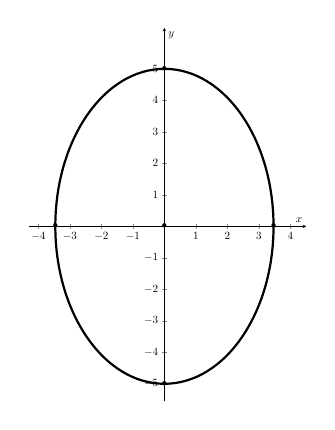
\begin{tikzpicture}[scale=0.4]
\begin{axis}[
x=1.0cm,y=1.0cm,
axis lines=middle,
xmin=-4.3,
xmax=4.5,
ymin=-5.56,
ymax=6.3, xlabel=$x$,ylabel=$y$,
xtick={-4.0,-3.0,...,4.0},
ytick={-5,-4,-3,-2.0,-1.0,...,5.0},]
\draw [rotate around={90.:(0.,0.)},line width=2.pt] (0.,0.) ellipse (5cm and 3.4641 cm);
\draw(0,5)node{$\bullet$};
\draw(0,-5)node{$\bullet$};
\draw(3.4641,0)node{$\bullet$};
\draw(-3.4641,0)node{$\bullet$};
\draw(0,0)node{$\bullet$};
\end{axis}
\end{tikzpicture}
\end{center}
\end{enumerate}	
	\item 
\begin{enumerate}[k]
\item រកដែនកំណត់នៃអនុគមន៍ $f$\\
ដោយ $f(x)=\frac{x^2+x+4}{x+1}$\quad ;\ $f(x)$\ មានន័យលុះត្រាតែ \ $x+1\neq 0\quad \Leftrightarrow \ x\neq -1$\\
\textbf{ដូចនេះ}\ \fbox{ដែនកំណត់នៃអនុគមន៍ $f$ គឺ $D_f=\mathbb{R}-\{-1\}$}
\item គណនា $\lim_{x\to -1}f(x),\ \lim_{x\to \pm\infty}f(x)$ 
\begin{flalign*}
&\lim_{x\to -1}f(x)=\lim_{x\to -1}\frac{x^2+x+4}{x+1}=\pm\infty\quad\quad \textbf{ដូចនេះ}\ \fbox{$\lim_{x\to -1}f(x)=\pm\infty$}&\\
&\lim_{x\to \pm\infty}f(x)=\lim_{x\pm\infty}\frac{x^2+x-4}{x+1}=\lim_{x\to\pm\infty}\frac{x^2}{x}=\pm\infty\quad \textbf{ដូចនេះ}\ \fbox{$\lim_{x\to\pm\infty}f(x)=\pm\infty$}
\end{flalign*}
\item សរសេរសមីការអាស៊ីមតូតឈរ និង អាស៊ីមតូតទ្រេតនៃក្រាប $C$ 
\begin{itemize}
\item ដោយ $\lim_{x\to -1}f(x)=\pm\infty $\quad \textbf{ដូចនេះ}\ \fbox{បន្ទាត់ $x=-1$ ជាអាស៊ីមតូតឈរ }
\item $f(x)=\frac{x^2+x+4}{x+1}=x+\frac{4}{x+1}$\quad ដោយ \ $\lim_{x\to \pm\infty}\frac{4}{x+1}=0$ \quad \textbf{ដូចនេះ} \ \fbox{បន្ទាត់ $y=x$ ជាអាស៊ីមតូតទ្រេត}
\end{itemize}
\item  សិក្សាសញ្ញាដេរីវេ $f'(x)$ នៃអនុគមន៍ $f$
\begin{flalign*}
f'(x)&=\left(\frac{x^2+x+4}{x+1}\right)'=\frac{\left(x^2+x+4\right)'(x+1)-(x+1)'\left(x^2+x+4\right)}{(x+1)^2}=\frac{(2x+1)(x+1)-\left(x^2+x+4\right)}{(x+1)^2}&\\
&=\frac{2x^2+2x+x+1-x^2-x-4}{(x+1)^2}=\frac{x^2+2x-3}{(x+1)^2}\\
f'(x)&=0\quad \Leftrightarrow\ x^2+2x-3=0\quad \text{មានឫស} \ x_1=1;\ x_2=-3
\end{flalign*}
\newpage 
តារាងសញ្ញាដេរីវេ $f'(x)$
\\[0.2cm]
\begin{tikzpicture}[scale=0.5]
   \tkzTabInit{$x$ / 1.5 , $f'(x)$ / 2}{$\ \ -\infty$ , $-3$,$-1$,$1$, $+\infty\ \ $}
   \tkzTabLine{, +, z, - ,d,-, z,+ }
\end{tikzpicture}\\
 បរមាធៀប 
\begin{itemize}
\item ត្រង់ $x=-3;\ f'(x)=0$ ប្តូរសញ្ញាពី $+$ ទៅ $-$ គេបាន $f$ មានអតិបរមាធៀបមួយ គឺ $f(-3)=\frac{(-3)^2-3+4}{-3+1}=-5$
\item ត្រង់ $x=1;\ f'(x)=0$ ប្តូរសញ្ញាពី $-$ ទៅ $+$ គេបាន $f$ មានអប្បបរមាធៀបមួយ គឺ $f(1)=\frac{1^2+1+4}{1+1}=3$
\end{itemize}
\item សង់តារាងអថេរភាព អាស៊ីមតូត និង ក្រាប $C$ នៃអនុគមន៍ $f$ 
\begin{itemize}
\item តារាងអថេរភាពនៃ $f$\\[0.2cm]
\begin{tikzpicture}[scale=0.5]
\begin{scriptsize}
   \tkzTabInit{$x$ / 1 , $f'(x)$ / 1.25, $f(x)$/3}{$\ \ -\infty$ , $-3$,$-1$,$1$, $+\infty\ \ $}
   \tkzTabLine{, +, z, - ,d,-, z,+ }
   \tkzTabVar{-/ $\ \ \ \  -\infty$, +/$-5$, -D+/ $-\infty$ /$+\infty$, -/ $3$ , +/ $+\infty\ \ \ \ $}
\end{scriptsize}
\end{tikzpicture}
\item ក្រាប $C$  
\begin{itemize}
\item $(C)\cap (y'oy)$\ ពេល $x=0$\quad គេបាន $y=\frac{0^2+0+4}{0+1}=4$
\end{itemize}
\begin{center}
\definecolor{qqwuqq}{rgb}{0.,0.39215686274509803,0.}
\begin{tikzpicture}[scale=0.7]
\draw(1,15)node{$
\begin{array}{l}
(d):\ y=x\\
\begin{tabular}{c|cc}
$x$&$0$&$1$\\
\hline 
$y$&$0$&$1$
\end{tabular}
\end{array}
$};
\begin{axis}[
x=1.0cm,y=1.0cm,
axis lines=middle,
xmin=-9,
xmax=7,
ymin=-10,
ymax=9,
xlabel=$x$,ylabel=$y$,
xtick={-8,-7.0,...,6.0},
ytick={-10,-9,...,8}]
\draw[line width=1.pt,color=qqwuqq,smooth,samples=100,domain=-8:5.8] plot(\x,{((\x)^(2)+(\x)+4)/((\x)+1)});
\draw [line width=1.pt,domain=-8.:6.] plot(\x,{\x});
\draw(6,6)node[right=-0.5cm]{$(d)$};
\draw(3.5,5)node[color=qqwuqq]{$(c)$};
\draw(-2,2)node[color=qqwuqq]{$x=-1$};
\draw [dashed](1,0)--(1,3)node{$\bullet$}--(0,3); 
\draw [dashed](-3,0)--(-3,-5)node{$\bullet$}--(0,-5); 
\draw [dashed](1,0)--(1,1)node{$\bullet$}--(0,1); 
\draw (0,4)node{$\bullet$};
\end{axis}
\end{tikzpicture}
\end{center}
\end{itemize}
\end{enumerate}		
\end{enumerate}





\newpage 
\maketitle 
    \borderline{វិញ្ញាសាទី១០}


\begin{enumerate}[I]
\item (១០ពិន្ទុ) ក្នុងថតតុមួយមានសៀវភៅគណិតវិទ្យា $7$ ក្បាល និងសៀវភៅភាសាខ្មែរ $5$ ក្បាល។  សិស្សម្នាក់បានយកសៀវភៅ $4$ ក្បាល ព្រមគ្នាចេញពីថតតុដោយចៃដន្យ។
\begin{enumerate}[k]
\item រកប្រូបាបដែល «សិស្សយកបានសៀវភៅគណិតវិទ្យាទាំង $4$ ក្បាល» ។
\item រកប្រូបាបដែល «សិស្សយកបានសៀវភៅភាសាខ្មែរ $1$ ក្បាលយ៉ាងតិច» ។
\end{enumerate}
\item (១០ពិន្ទុ) គណនាលីមីត៖
\begin{enumerate}[k,3]
\item $\lim_{x\to 1}\frac{x^2-1}{x^2-3x+2}$
\item $\lim_{x\to 2}\frac{2-\sqrt{2+x}}{x^2-4}$
\item  $\lim_{x\to 0}\frac{x}{\sqrt{3}-\sqrt{x+3}}$
\end{enumerate} 
\item (១០ពិន្ទុ) គណនាអាំងតេក្រាលខាងក្រោម៖
\begin{enumerate}[k,3]
\item $\int_0^2 \left(\frac{1}{1-x}-3x+1\right)dx$
\item $\int_1^2 \left(\frac{2}{x^2}+3-x\right)dx$
\item $\int_1^3 \left(\frac{x^2-3x+2}{2-x}\right) dx$
\end{enumerate}
\item (១៥ពិន្ទុ) រកសមីការស្តង់ដានៃអេលីបមួយដែលមានកំណុំមួយនៅត្រង់ចំណុច $(0,2)$ និងកំពូលពីរនៅត្រង់ចំណុច $(0,-3)$ និង $(0,3)$។ រួចរកប្រវែងអ័ក្សតូច ប្រវែងអ័ក្សធំ និងសង់អេលីប។
\item (៣០ពិន្ទុ) គេមានអនុគមន៍ $f$ កំណត់ដោយ $y=f(x)=\frac{x^2-4}{x-1}$   មានក្រាបតំណាង $C$ ។
\begin{enumerate}[m]
\item ចូររកដែនកំណត់នៃអនុគមន៍ $f$ ។
\item គណនា $\lim_{x\to 1}f(x);\ \lim_{x\to \pm\infty}f(x)$ ។ រួចទាញរកសមីការអាស៊ីមតូតឈរ។
\item បង្ហាញថា $f(x)=x+1-\frac{3}{x-1}$ ។ រួចបង្ហាញថាបន្ទាត់ $d$ ដែលមានសមីការ $y=x+1$ ជាអាស៊ីមតូតទ្រេតនៃក្រាប $C$ ខាង $\pm\infty$ ។
\item គណនាដេរីវេ $f'(x)$ និងសិក្សាសញ្ញាដេរីវេ $f'(x)$ ។
\item 
\begin{enumerate}[k]
\item សង់តារាងអថេរភាពនៃ $f$។ 
\item សិក្សាទីតាំងធៀបរវាងក្រាប $C$ និងបន្ទាត់ $d$ ។
\item សង់ក្រាប $C$ និងបន្ទាត់ $d$ ក្នងតម្រុយតែមួយ។
\end{enumerate}
\end{enumerate}
\end{enumerate}
 \newpage 
\borderline{ចម្លើយ}

\begin{enumerate}[I]
\item 
\begin{enumerate}[k]
\item រកប្រូបាបដែល «សិស្សយកបានសៀវភៅគណិតវិទ្យាទាំង $4$ ក្បាល» 
\\ តាង $A:$ «សិស្សយកបានសៀវភៅគណិតវិទ្យាទាំង $4$ ក្បាល»
\begin{flalign*}
\text{តាមរូបមន្ត}\ P(A)=\frac{n(A)}{n(S)}\quad \text{ដោយ}\ n(A)&=C(7,4)=\frac{7!}{3!4!}=\frac{7\times 6\times 5\times 4!}{3\times 2\times 1\times 4!}=35&\\
n(S)&=C(12,4)=\frac{12!}{8!4!}=\frac{12\times 11\times 10\times 9\times 8!}{8!\times 4\times 3\times 2\times 1}=495
\end{flalign*}
គេបាន \ $P(A)=\frac{n(A)}{n(S)}=\frac{35}{495}=\frac{7}{99}$\quad \textbf{ដូចនេះ}\ \fbox{$P(A)=\frac{7}{99}$}
\item រកប្រូបាបដែល «សិស្សយកបានសៀវភៅភាសាខ្មែរ $1$ ក្បាលយ៉ាងតិច» \\
តាង \ $B:$ «សិស្សយកបានសៀវភៅភាសាខ្មែរ $1$ ក្បាលយ៉ាងតិច» 
\begin{flalign*}
&\text{តាមរូបមន្ត}\ P(B)=1-P(A)=1-\frac{7}{99}=\frac{99-7}{99}=\frac{92}{99} \quad \textbf{ដូចនេះ}\ \fbox{$P(B)=\frac{92}{99}$}&
\end{flalign*}
\end{enumerate}
\item គណនាលីមីត៖
\begin{enumerate}[k]
\item $\lim_{x\to 1}\frac{x^2-1}{x^2-3x+2}$\quad (មានរាងមិនកំណត់$\tfrac{0}{0}$)
\begin{flalign*}
&=\lim_{x\to 1}\frac{(x-1)(x+1)}{(x-1)(x-2)}=\lim_{x\to 1}\frac{x+1}{x-2}=\frac{1+1}{1-2}=-2\quad \textbf{ដូចនេះ}\ \fbox{$\lim_{x\to 1}\frac{x^2-1}{x^2-3x+2}=-2$}&
\end{flalign*}
\item $\lim_{x\to 2}\frac{2-\sqrt{2+x}}{x^2-4}$\quad (មានរាងមិនកំណត់$\tfrac{0}{0}$)
\begin{flalign*}
&=\lim_{x\to 2}\frac{\left(2-\sqrt{2+x}\right)\left(2+\sqrt{2+x}\right)}{(x-2)(x+2)\left(2+\sqrt{2+x}\right)}=\lim_{x\to 2}\frac{4-(2+x)}{(x-2)(x+2)\left(2+\sqrt{2+x}\right)}=\lim_{x\to 2}\frac{-(x-2)}{(x-2)(x+2)\left(2+\sqrt{2+x}\right)}&\\
&=\frac{-1}{(2+2)\left(2+\sqrt{2+2}\right)}=-\frac{1}{16}\quad \textbf{ដូចនេះ}\ \fbox{$\lim_{x\to 2}\frac{2-\sqrt{2+x}}{x^2-4}=-\frac{1}{16}$}
\end{flalign*}
\item  $\lim_{x\to 0}\frac{x}{\sqrt{3}-\sqrt{x+3}}$\quad (មានរាងមិនកំណត់$\tfrac{0}{0}$)
\begin{flalign*}
&=\lim_{x\to 0}\frac{x\left(\sqrt{3}+\sqrt{x+3}\right)}{\left(\sqrt{3}-\sqrt{x+3}\right)\left(\sqrt{3}+\sqrt{x+3}\right)}=\lim_{x\to 0}\frac{x\left(\sqrt{3}+\sqrt{x+3}\right)}{3-(x+3)}=\lim_{x\to 0}\frac{x\left(\sqrt{3}+\sqrt{x+3}\right)}{-x}=\frac{\sqrt{3}+\sqrt{0+3}}{-1}&
\end{flalign*}
\textbf{ដូចនេះ}\ \fbox{$ \lim_{x\to 0}\frac{x}{\sqrt{3}-\sqrt{x+3}}=-2\sqrt{3}$}
\end{enumerate} 
\item គណនាអាំងតេក្រាល៖
\begin{enumerate}[k]
\item $\int_0^2 \left(\frac{1}{1-x}-3x+1\right)dx=\left[-\ln |1-x|-\frac{3x^2}{2}+x\right]_0^2=-\ln |1-2|-\frac{3(2)^2}{2}+2-\left(-\ln |1-0|-\frac{3(0)^2}{0}+0\right)$\\[0.2cm]
 \hphantom{$\int_0^2 \left(\frac{1}{1-x}-3x+1\right)dx$} 
 $=-\ln 1-6+2-0=-4$\\[0.2cm]
  \textbf{ដូចនេះ}\ \fbox{$\int_0^2 \left(\frac{1}{1-x}-3x+1\right)dx=-4$}
\item $\int_1^2 \left(\frac{2}{x^2}+3-x\right)dx=\left[-\frac{2}{x}+3x-\frac{x^2}{2}\right]_1^2=-\frac{2}{2}+3(2)-\frac{2^2}{2}-\left(-\frac{2}{1}+3(1)-\frac{1^2}{2}\right)=3-\frac{1}{2}=\frac{5}{2}$\\[0.2cm]
\textbf{ដូចនេះ}\ \fbox{ $\int_1^2 \left(\frac{2}{x^2}+3-x\right)dx=\frac{5}{2}$}
\newpage 
\item $\int_1^3 \left(\frac{x^2-3x+2}{2-x}\right) dx =\int_1^3\left( \frac{(x-1)(x-2)}{-(x-2)}\right) dx=\int_1^3\left(-x+2\right)dx=\left[-\frac{x^2}{2}+2x\right]_1^3 =-\frac{3^2}{2}+2(3)-\left(-\frac{1^2}{2}+2(1)\right)$\\[0.2cm]
\hphantom{$\int_1^3 \left(\frac{x^2-3x+2}{2-x}\right) dx $} $=-\frac{9}{2}+6+\frac{1}{2}-2=-4+4=0$\\[0.2cm]
\textbf{ដូចនេះ}\ \fbox{$\int_1^3 \left(\frac{x^2-3x+2}{2-x}\right) dx=0$}
\end{enumerate}
\item  \begin{itemize}[2]
\item រកសមីការស្តង់ដានៃអេលីបដែលមានកំណុំ $(0,2)$ និងកំពូលពីរ $(0,-3)$ និង $(0,3)$
\\ ដោយ អាប់ស៊ីសនៃកំពូល និងកំណុំថេរ គេបាន អ័ក្សធំនៃអេលីបជាអ័ក្សឈរ 
\begin{itemize}
\item សមីការស្តង់ដានៃអេលីបគឺ $\frac{(x-h)^2}{b^2}+\frac{(y-k)^2}{a^2}=1$
\item កំពូល $(0,-3);\ (0,3)$ គឺ $V_1(h,k-a);\ V_2(h,k+a)$ \\ គេបាន $h=0;\ k-a=-3;\quad k+a=3$ 
\begin{flalign*} & 
\begin{array}{l}
\left\{\begin{array}{l}
k-a=-3\\
\underline{k+a=3}
\end{array}\right.\\
\ \ \ 
 2k=0\quad \Rightarrow\ k=0;\quad \Rightarrow \ a=3
\end{array} &
\end{flalign*}
\item កំណុំ$(0,2)$ គឺ$F(h,k+c)  \Rightarrow h=0;\ k+c=2\Rightarrow c=2$
\item $c^2=a^2-b^2\quad \Rightarrow\ b^2=a^2-c^2=3^2-2^2=5$
\end{itemize}
\textbf{ដូចនេះ}\ \fbox{សមីការអេលីបគឺ $\frac{x^2}{5}+\frac{y^2}{9}=1$}
\item  រួចរកប្រវែងអ័ក្សតូច ប្រវែងអ័ក្សធំ និងសង់អេលីប
\begin{itemize}
\item ប្រវែងអ័ក្សតូច $=2b=2(\sqrt{5})$
\item ប្រវែងអ័ក្សធំ $=2a=2(3)=6$
\item សង់អេលីប 
\begin{center}
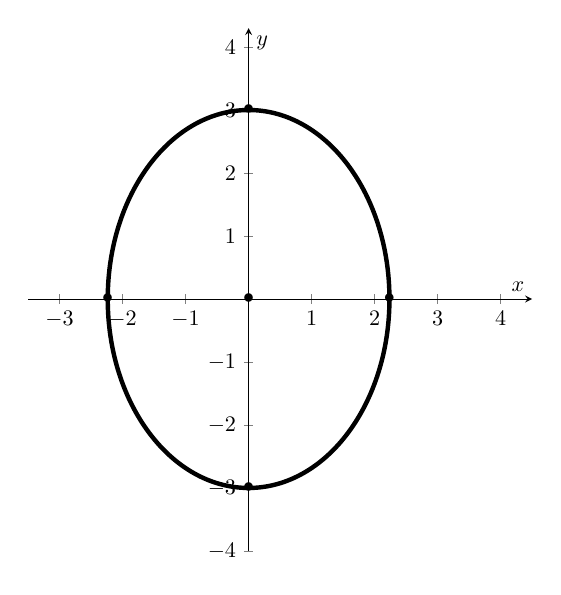
\begin{tikzpicture}[scale=0.8]
\begin{axis}[
x=1.0cm,y=1.0cm,
axis lines=middle,
xmin=-3.5,
xmax=4.5,
ymin=-4,
ymax=4.3, xlabel=$x$,ylabel=$y$,
xtick={-3.0,...,4.0},
ytick={-4,-3,-2.0,-1.0,...,4.0},]
\draw [rotate around={90.:(0.,0.)},line width=2.pt] (0.,0.) ellipse (3.cm and 2.23606797749979cm);
\draw(0,3)node{$\bullet$};
\draw(0,-3)node{$\bullet$};
\draw(2.236,0)node{$\bullet$};
\draw(-2.236,0)node{$\bullet$};
\draw(0,0)node{$\bullet$};
\end{axis}
\end{tikzpicture}
\end{center}
\end{itemize}
\end{itemize}
\item  
\begin{enumerate}[m]
\item រកដែនកំណត់នៃអនុគមន៍ $f$ 
\\ ដោយ $y=f(x)=\frac{x^2-4}{x-1}$\quad ;\ $f(x)$\   មានន័យលុះត្រាតែ $x-1\neq 0\quad \Rightarrow\ x\neq 1$\\[0.2cm]
\textbf{ដូចនេះ}\ \fbox{ដែនកំណត់នៃ$f$ គឺ $D_f=\mathbb{R}-\{1\}$}
\item គណនា $\lim_{x\to 1}f(x);\ \lim_{x\to \pm\infty}f(x)$  រួចទាញរកសមីការអាស៊ីមតូតឈរ
\begin{flalign*}
&\lim_{x\to 1}f(x)= \lim_{x\to 1}\frac{x^2-4}{x-1}= \pm \infty\quad\quad\quad \quad \quad \quad\quad \ \  \textbf{ដូចនេះ}\ \fbox{$\lim_{x\to 1}f(x)=\pm\infty$}& \\
&\lim_{x\to \pm \infty}f(x)=\lim_{x\to \pm\infty}\frac{x^2-4}{x-1}=\lim_{x\to \pm\infty}\frac{x^2}{x}=\pm\infty\quad \textbf{ដូចនេះ}\ \fbox{$\lim_{x\to \pm\infty} f(x)=\pm\infty $}
\end{flalign*} 
ដោយ $\lim_{x\to 1}f(x)=\pm\infty$\quad \textbf{ដូចនេះ}\ \fbox{បន្ទាត់ $x=1$ ជាអាស៊ីមតូតឈរ }
\item បង្ហាញថា $f(x)=x+1-\frac{3}{x-1}$  
\begin{flalign*}
\text{ដោយ}\ x+1-\frac{3}{x-1}&=\frac{(x+1)(x-1)-3}{x-1}=\frac{x^2-1-3}{x-1}=\frac{x^2-4}{x-1}=f(x)\quad \textbf{ដូចនេះ}\ \fbox{$f(x)=x+1-\frac{3}{x-1}$}& 
\end{flalign*}
បង្ហាញថាបន្ទាត់ $d$ ដែលមានសមីការ $y=x+1$ ជាអាស៊ីមតូតទ្រេតនៃក្រាប $C$ ខាង $\pm\infty$ 
\begin{flalign*}
&\text{ដោយ}\ \lim_{x\to \pm\infty} \frac{-3}{x-1}=0\quad \textbf{ដូចនេះ}\ \fbox{បន្ទាត់ $y=x+1$ ជាអាស៊ីមតូតទ្រេត}&
\end{flalign*}
\newpage
\item 
\begin{itemize}
\item គណនាដេរីវេ $f'(x)$ និងសិក្សាសញ្ញាដេរីវេ $f'(x)$ 
\begin{flalign*}
f'(x)&=\left(\frac{x^2-4}{x-1}\right)'=\frac{\left(x^2-4\right)'(x-1)-(x-1)'\left(x^2-4\right)}{(x-1)^2}=\frac{2x(x-1)-\left(x^2-4\right)}{(x-1)^2} =\frac{x^2-2x+4}{(x-1)^2}&\\
f'(x)&=0\quad \Leftrightarrow\ x^2-2x+4=0\quad ;\ \Delta = b^2-4ac =(-2)^2-4(1)4=-12<0;\ f'(x)\ \text{យកសញ្ញាតាមមេគុណ} a
\end{flalign*}
\item តារាងសញ្ញា $f'(x)$		
\\[0.2cm]
\begin{tikzpicture}[scale=0.5]
   \tkzTabInit{$x$ / 1.5 , $f'(x)$ / 2}{$\ \ -\infty$ , $1$, $+\infty\ \ $}
   \tkzTabLine{,+,d,+, }
\end{tikzpicture}	
\begin{itemize}
\item $f'(x)>0;\ $ ពេល $x\in (-\infty , 1)\cup (1,+\infty)$
\end{itemize}
\end{itemize}
\item 
\begin{enumerate}[k]
\item សង់តារាងអថេរភាពនៃ $f$
\\[0.2cm]
\begin{tikzpicture}[scale=0.8]
   \tkzTabInit{$x$ / 1 , $f'(x)$ / 1.25, $f(x)$/2}{$\ \ -\infty$ ,$1$, $+\infty\ \ $}
   \tkzTabLine{, +, d, + , }
   \tkzTabVar{-/ $-\infty$,  +D-/ $+\infty$ /$-\infty$, +/ $+\infty$ }
\end{tikzpicture}
\item សិក្សាទីតាំងធៀបរវាងក្រាប $C$ និងបន្ទាត់ $d$ \\
$(C):\ y=x+1-\frac{3}{x-1};\quad (d):\ y= x+1 $ \ គេបាន $y_c-y_d=x+1-\frac{3}{x-1}-(x+1)=-\frac{3}{x-1}$
\begin{itemize}
\item $y_c-y_d>0\quad \Leftrightarrow \ -\frac{3}{x-1}>0\quad\Leftrightarrow \ x-1<0\ \Leftrightarrow\ x<1$\quad \textbf{ដូចនេះ}\ \fbox{$C$ ស្ថិតនៅលើ $d$ ពេល $x<1$}
\item $y_c-y_d<0\quad \Leftrightarrow \ -\frac{3}{x-1}<0\quad\Leftrightarrow \ x-1>0\ \Leftrightarrow\ x>1$\quad \textbf{ដូចនេះ}\ \fbox{$C$ ស្ថិតនៅក្រោម $d$ ពេល $x>1$}
\end{itemize}
\item សង់ក្រាប $C$ និងបន្ទាត់ $d$ ក្នងតម្រុយតែមួយ
\begin{itemize}
\item  $(C)\cap (y'oy)$ គឺ $x=0;\quad \Rightarrow\ y=\frac{0^2-4}{0-1}=4$ 
\item  $(C)\cap (x'ox)$ គឺ $y=0;\quad \Rightarrow\ x^2-4=0\quad \Rightarrow\ x=\pm 2 $
\end{itemize}
\begin{center}
\definecolor{qqwuqq}{rgb}{0.,0.39215686274509803,0.}
\begin{tikzpicture}[scale=0.56]
\begin{scriptsize}[scale=0.5]
\draw(5,15)node{$
\begin{array}{l}
(d):\ y=x+1\\
\begin{tabular}{c|cc}
$x$&$0$&$-1$\\
\hline 
$y$&$1$&$0$
\end{tabular}
\end{array}
$};
\end{scriptsize}
\begin{axis}[
x=1.0cm,y=1.0cm,
axis lines=middle,
xmin=-8.5,
xmax=8.2,
ymin=-9,
ymax=8.5,
xlabel=$x$,ylabel=$y$,
xtick={-8,-7,-6.0,-5.0,...,6.0,7,8},
ytick={-8,-7,-6.0,-5.0,...,7.0},]
\draw[line width=1.pt,color=qqwuqq,smooth,samples=80,domain=-8:8] plot(\x,{((\x)^(2)-4)/((\x)-1)});
\draw [line width=1.pt,domain=-8.:8] plot(\x,{\x+1});
\draw(-6,-7)node{$(d):\ y=x+1$};
\draw(7,6)node[color=qqwuqq]{$(c)$};
\draw(1.62,8)node[color=qqwuqq]{$x=1$};
\draw (2,0)node{$\bullet$}; \draw (-2,0)node{$\bullet$}; \draw (0,4)node{$\bullet$}; 
\end{axis}
\end{tikzpicture}
\end{center}
\end{enumerate}
\end{enumerate}
\end{enumerate}



 
\newpage 
\maketitle 
\begin{center}
\kml
  វិញ្ញាសាទី១១ ({\kn ថ្នាក់សង្គម})\\ 
  \end{center}
    \borderline{សំណួរ}
    \begin{enumerate}[I]




\item (១៥ពិន្ទុ) អេលីប $\mathrm{E}$ មួយមានសមីការទូទៅ៖ $9x^2+4y^2+18x-24y+9=0$ ។ 
\begin{enumerate}[k]
\item រកសមីការស្តង់ដានៃអេលីប $\mathrm{E}$ ។
\item រកប្រវែងអ័ក្សធំ និង អ័ក្សតូច ហើយរកកូអរដោនេនៃ ផ្ចិត កំពូល និង កំណុំនៃអេលីប $\mathrm{E}$ ។
\end{enumerate}
\item (៣០ពិន្ទុ)  អនុគមន៍ $f$ កំណត់ចំពោះ $x\neq -2,\ \ x\neq 2$ ដោយ $y=f(x)=\frac{x^2}{4-x^2}$ និងមានក្រាប $C$ ។ 
		\begin{enumerate}[k]
		\item គណនា$\lim_{x\to -2}f(x), \lim_{x\to 2}f(x)$ និង$\lim_{x\to \pm \infty}f(x)$។   ទាញរកសមីការអាស៊ីមតូតឈរ និងអាស៊ីមតូតទ្រេតនៃក្រាប$C$ ។
		\item សិក្សាសញ្ញានៃដេរីវេ $f'(x)$ និងសង់តារាងអថេរភាពនៃ $f$ ។
		\item គណនា $f(-3)$ និង $f(3)$ ហើយក្រាប $C$ នៃអនុគមន៍ $f$ ។
		\end{enumerate}

\end{enumerate}

 \newpage 
\borderline{ចម្លើយ}\\
{\color{white}.}\dotfill\\
{\color{white}.}\dotfill\\
{\color{white}.}\dotfill
\\
{\color{white}.}\dotfill\\
{\color{white}.}\dotfill\\
{\color{white}.}\dotfill
\\
{\color{white}.}\dotfill\\
{\color{white}.}\dotfill\\
{\color{white}.}\dotfill
\\
{\color{white}.}\dotfill\\
{\color{white}.}\dotfill\\
{\color{white}.}\dotfill
\\
{\color{white}.}\dotfill\\
{\color{white}.}\dotfill\\
{\color{white}.}\dotfill
\\
{\color{white}.}\dotfill\\
{\color{white}.}\dotfill\\
{\color{white}.}\dotfill
\\
{\color{white}.}\dotfill\\
{\color{white}.}\dotfill\\
{\color{white}.}\dotfill
\\
{\color{white}.}\dotfill\\
{\color{white}.}\dotfill\\
{\color{white}.}\dotfill
\\
{\color{white}.}\dotfill\\
{\color{white}.}\dotfill\\
{\color{white}.}\dotfill
\\
{\color{white}.}\dotfill\\
{\color{white}.}\dotfill\\
{\color{white}.}\dotfill\\
{\color{white}.}\dotfill\\
{\color{white}.}\dotfill\\
{\color{white}.}\dotfill
\\
{\color{white}.}\dotfill\\
{\color{white}.}\dotfill\\
{\color{white}.}\dotfill
\\
{\color{white}.}\dotfill\\
{\color{white}.}\dotfill\\
{\color{white}.}\dotfill
\\
{\color{white}.}\dotfill\\
{\color{white}.}\dotfill\\
{\color{white}.}\dotfill
\\
{\color{white}.}\dotfill\\
{\color{white}.}\dotfill\\
{\color{white}.}\dotfill
\\
{\color{white}.}\dotfill 
\newpage 
\maketitle 
\begin{center}
\kml
  វិញ្ញាសាទី១២ ({\kn ថ្នាក់សង្គម})\\
  \end{center}
    \borderline{សំណួរ}
    
    \begin{enumerate}[I]
\item (១០ពិន្ទុ)  គណនាលីមីត៖

\begin{enumerate}[k,2]

\item   $\lim_{x\to 1}\frac{1-x^2}{x^2+2-3x}$
\end{enumerate}


\item (១០ពិន្ទុ)   គ្រូបន្ទុកថ្នាក់បានជ្រើសរើសប្រធានក្រុមវេនសំអាតថ្នាក់ថ្ងៃចំនួន $6$ នាក់នៃថ្នាក់រៀនមួយដែលមាន សិស្សប្រុសចំនួន$20$ នាក់ និងសិស្សស្រីចំនួន $15$នាក់ ។ គណនាប្រូបាបខាងក្រោម៖ 
\begin{enumerate}[A]
\item «ប្រធានក្រុមសុទ្ធតែប្រុស»
\item «ប្រធានក្រុមសុទ្ធតែស្រី»
\item «ប្រធានក្រុមមានប្រុស$3$ នាក់ និងស្រី$3$ នាក់» ។
\end{enumerate}
\item (១០ពិន្ទុ)  គេឲ្យ $\mathrm{A}(x)=\frac{x+1}{(x-1)^2}$ ចំពោះគ្រប់ $x\neq 1$ ។
\begin{enumerate}[k]
\item រកចំនួនពិត $a$ និង $b$ ដើម្បីឲ្យ $\mathrm{A}(x)=\frac{a}{x-1}+\frac{b}{(x-1)^2}$ ចំពោះគ្រប់ $x\neq 1$ ។
\item គណនា $\mathrm{I}(x)=\int\mathrm{A}(x)dx$ ។
\end{enumerate}


\item (៣០ពិន្ទុ) គេឲ្យអនុគមន៍ $f$ កំណត់ដោយ $f(x)=\frac{2x^2+3x-5}{x+2}$ ហើយមានក្រាប $C$ ។ 
\begin{enumerate}[k]
\item រកដែនកំណត់ និងសិក្សាសញ្ញាដេរីវេនៃអនុគមន៍$f$ ។
\item សរសេរសមីការអាស៊ីមតូតឈរ និងអាស៊ីមតូតទ្រេតនៃក្រាប $C$ ។
\item សង់តារាងអថេរភាពនៃអនុគន៍ $f$ និងសង់ក្រាប $C$ ។
\item ដោះស្រាយវិសមីការ $\frac{2x^2+3x-5}{x+2}<2x-1$ ដោយប្រើក្រាប$C$ ។
\end{enumerate}
\end{enumerate}

 \newpage 
\borderline{ចម្លើយ}\\
{\color{white}.}\dotfill\\
{\color{white}.}\dotfill\\
{\color{white}.}\dotfill
\\
{\color{white}.}\dotfill\\
{\color{white}.}\dotfill\\
{\color{white}.}\dotfill
\\
{\color{white}.}\dotfill\\
{\color{white}.}\dotfill\\
{\color{white}.}\dotfill
\\
{\color{white}.}\dotfill\\
{\color{white}.}\dotfill\\
{\color{white}.}\dotfill
\\
{\color{white}.}\dotfill\\
{\color{white}.}\dotfill\\
{\color{white}.}\dotfill
\\
{\color{white}.}\dotfill\\
{\color{white}.}\dotfill\\
{\color{white}.}\dotfill
\\
{\color{white}.}\dotfill\\
{\color{white}.}\dotfill\\
{\color{white}.}\dotfill
\\
{\color{white}.}\dotfill\\
{\color{white}.}\dotfill\\
{\color{white}.}\dotfill
\\
{\color{white}.}\dotfill\\
{\color{white}.}\dotfill\\
{\color{white}.}\dotfill
\\
{\color{white}.}\dotfill\\
{\color{white}.}\dotfill\\
{\color{white}.}\dotfill\\
{\color{white}.}\dotfill\\
{\color{white}.}\dotfill\\
{\color{white}.}\dotfill
\\
{\color{white}.}\dotfill\\
{\color{white}.}\dotfill\\
{\color{white}.}\dotfill
\\
{\color{white}.}\dotfill\\
{\color{white}.}\dotfill\\
{\color{white}.}\dotfill
\\
{\color{white}.}\dotfill\\
{\color{white}.}\dotfill\\
{\color{white}.}\dotfill
\\
{\color{white}.}\dotfill\\
{\color{white}.}\dotfill\\
{\color{white}.}\dotfill
\\
{\color{white}.}\dotfill 


\newpage 
ក្នុងប្លង់ប្រដាប់ដោយតម្រុយអរតូណរមេ $\left(o,\overrightarrow{i},\overrightarrow{j}\right)$ : (ឯកតា $2\mathrm{cm}$) ។
		គេមានអនុគមន៍ $f$ និង $g$ កំណត់លើសំណុំចំនួនពិត $\mathbb{R}$  ដោយ៖
$f(x)=x-e^x$ និង  $g(x)=(1-x)e^x$ និង គេតាង $(c)$  និង $\left(c'\right)$  ក្រាបនៃអនុគមន៍  $f$ និង $g$ 		នេះ។
		\begin{enumerate}[k]
		\item \begin{enumerate}[a]
					\item  កំណត់លីមីតនៃអនុគមន៍ $f$ និង $g$  ត្រង់ $+\infty$  និង $-\infty$  ។
					\item បង្ហាញថាបន្ទាត់ $(\Delta)$ ដែលមានសមីការ $y=x$  ជាអាស៊ីមតូតនៃក្រាប $(c)$  ។
					\item សិក្សាអថេរភាពនៃអនុគមន៍ $f$ និង អនុគមន៍ $g$ លើ $\mathbb{R}$ ។
					\item សង់តារាងអថេរភាពនៃអនុគមន៍ $f$ និង អនុគមន៍ $g$ ។
		\end{enumerate}
	\item ចំពោះគ្រប់ចំនួនពិត $x$ គេតាង $h(x)=f(x)-g(x)$  ។
			\begin{enumerate}[a]
			\item បង្ហាញថាគ្រប់ចំនួនពិត $x,\ h'(x)=1-g(x)$ ។
			\item ទាញយកទិសដៅអថេរភាពនៃអនុគមន៍  $h$ លើសំណុំចំនួនពិត។
			\item ស្រាយបញ្ជាក់ថាក្រាប $(c)$ និង $(c')$ មានចំណុចប្រសព្វតែមួយគត់ដែលមានអាប់ស៊ីសរបស់វាតាងដោយ $\alpha$ នៅលើចន្លោះ $[1,2]$ ។  
			\item សិក្សាទៅតាមតម្លៃនៃ $\alpha$  ទីតាំងធៀបគ្នារវាង $(c)$ និង $(c')$ ។
			\end{enumerate}
\item សង់បន្ទាត់ $(\Delta)$ និងក្រាប $(c)$ និង $(c')$ ។
\item ចំពោះគ្រប់ចំនួនពិត $x$ គេតាង $\theta  (x)=\int_0^xh(t)dt$ ។ 
		\begin{enumerate}[a]
		\item ប្រើអាំងតេក្រាលដោយផ្នែកគណនា $\theta (x)$ ។
		\item ទាញយកជារាងកន្សោមសនិទាននៃ  $\alpha$ ផ្ទៃក្រទ្បាជា $\mathrm{cm^2}$  នៃដែនដែលអមដោយក្រាប $(c)$ និង $(c')$,\ អ័ក្សអរដោនេ និង បន្ទាត់ដែលមានសមីការ $x=\alpha$ ។
		\end{enumerate}
\end{enumerate}	


           \end{document}
